% Generated by Sphinx.
\def\sphinxdocclass{report}
\documentclass[a4paper,10pt,english]{sphinxmanual}
\usepackage[utf8]{inputenc}
\DeclareUnicodeCharacter{00A0}{\nobreakspace}
\usepackage{cmap}
\usepackage[T1]{fontenc}
\usepackage{babel}
\usepackage{times}
\usepackage[Bjarne]{fncychap}
\usepackage{longtable}
\usepackage{sphinx}
\usepackage{multirow}
\usepackage{amsmath, amssymb}


\title{HARDPIG}
\date{March 01, 2014}
\release{1.0a}
\author{Timothy Kam and Ronald Stauber}
\newcommand{\sphinxlogo}{
\includegraphics{logo.png}\par}
\renewcommand{\releasename}{Release}
\makeindex

\makeatletter
\def\PYG@reset{\let\PYG@it=\relax \let\PYG@bf=\relax%
    \let\PYG@ul=\relax \let\PYG@tc=\relax%
    \let\PYG@bc=\relax \let\PYG@ff=\relax}
\def\PYG@tok#1{\csname PYG@tok@#1\endcsname}
\def\PYG@toks#1+{\ifx\relax#1\empty\else%
    \PYG@tok{#1}\expandafter\PYG@toks\fi}
\def\PYG@do#1{\PYG@bc{\PYG@tc{\PYG@ul{%
    \PYG@it{\PYG@bf{\PYG@ff{#1}}}}}}}
\def\PYG#1#2{\PYG@reset\PYG@toks#1+\relax+\PYG@do{#2}}

\expandafter\def\csname PYG@tok@gd\endcsname{\def\PYG@tc##1{\textcolor[rgb]{0.63,0.00,0.00}{##1}}}
\expandafter\def\csname PYG@tok@gu\endcsname{\let\PYG@bf=\textbf\def\PYG@tc##1{\textcolor[rgb]{0.50,0.00,0.50}{##1}}}
\expandafter\def\csname PYG@tok@gt\endcsname{\def\PYG@tc##1{\textcolor[rgb]{0.00,0.27,0.87}{##1}}}
\expandafter\def\csname PYG@tok@gs\endcsname{\let\PYG@bf=\textbf}
\expandafter\def\csname PYG@tok@gr\endcsname{\def\PYG@tc##1{\textcolor[rgb]{1.00,0.00,0.00}{##1}}}
\expandafter\def\csname PYG@tok@cm\endcsname{\let\PYG@it=\textit\def\PYG@tc##1{\textcolor[rgb]{0.25,0.50,0.56}{##1}}}
\expandafter\def\csname PYG@tok@vg\endcsname{\def\PYG@tc##1{\textcolor[rgb]{0.73,0.38,0.84}{##1}}}
\expandafter\def\csname PYG@tok@m\endcsname{\def\PYG@tc##1{\textcolor[rgb]{0.13,0.50,0.31}{##1}}}
\expandafter\def\csname PYG@tok@mh\endcsname{\def\PYG@tc##1{\textcolor[rgb]{0.13,0.50,0.31}{##1}}}
\expandafter\def\csname PYG@tok@cs\endcsname{\def\PYG@tc##1{\textcolor[rgb]{0.25,0.50,0.56}{##1}}\def\PYG@bc##1{\setlength{\fboxsep}{0pt}\colorbox[rgb]{1.00,0.94,0.94}{\strut ##1}}}
\expandafter\def\csname PYG@tok@ge\endcsname{\let\PYG@it=\textit}
\expandafter\def\csname PYG@tok@vc\endcsname{\def\PYG@tc##1{\textcolor[rgb]{0.73,0.38,0.84}{##1}}}
\expandafter\def\csname PYG@tok@il\endcsname{\def\PYG@tc##1{\textcolor[rgb]{0.13,0.50,0.31}{##1}}}
\expandafter\def\csname PYG@tok@go\endcsname{\def\PYG@tc##1{\textcolor[rgb]{0.20,0.20,0.20}{##1}}}
\expandafter\def\csname PYG@tok@cp\endcsname{\def\PYG@tc##1{\textcolor[rgb]{0.00,0.44,0.13}{##1}}}
\expandafter\def\csname PYG@tok@gi\endcsname{\def\PYG@tc##1{\textcolor[rgb]{0.00,0.63,0.00}{##1}}}
\expandafter\def\csname PYG@tok@gh\endcsname{\let\PYG@bf=\textbf\def\PYG@tc##1{\textcolor[rgb]{0.00,0.00,0.50}{##1}}}
\expandafter\def\csname PYG@tok@ni\endcsname{\let\PYG@bf=\textbf\def\PYG@tc##1{\textcolor[rgb]{0.84,0.33,0.22}{##1}}}
\expandafter\def\csname PYG@tok@nl\endcsname{\let\PYG@bf=\textbf\def\PYG@tc##1{\textcolor[rgb]{0.00,0.13,0.44}{##1}}}
\expandafter\def\csname PYG@tok@nn\endcsname{\let\PYG@bf=\textbf\def\PYG@tc##1{\textcolor[rgb]{0.05,0.52,0.71}{##1}}}
\expandafter\def\csname PYG@tok@no\endcsname{\def\PYG@tc##1{\textcolor[rgb]{0.38,0.68,0.84}{##1}}}
\expandafter\def\csname PYG@tok@na\endcsname{\def\PYG@tc##1{\textcolor[rgb]{0.25,0.44,0.63}{##1}}}
\expandafter\def\csname PYG@tok@nb\endcsname{\def\PYG@tc##1{\textcolor[rgb]{0.00,0.44,0.13}{##1}}}
\expandafter\def\csname PYG@tok@nc\endcsname{\let\PYG@bf=\textbf\def\PYG@tc##1{\textcolor[rgb]{0.05,0.52,0.71}{##1}}}
\expandafter\def\csname PYG@tok@nd\endcsname{\let\PYG@bf=\textbf\def\PYG@tc##1{\textcolor[rgb]{0.33,0.33,0.33}{##1}}}
\expandafter\def\csname PYG@tok@ne\endcsname{\def\PYG@tc##1{\textcolor[rgb]{0.00,0.44,0.13}{##1}}}
\expandafter\def\csname PYG@tok@nf\endcsname{\def\PYG@tc##1{\textcolor[rgb]{0.02,0.16,0.49}{##1}}}
\expandafter\def\csname PYG@tok@si\endcsname{\let\PYG@it=\textit\def\PYG@tc##1{\textcolor[rgb]{0.44,0.63,0.82}{##1}}}
\expandafter\def\csname PYG@tok@s2\endcsname{\def\PYG@tc##1{\textcolor[rgb]{0.25,0.44,0.63}{##1}}}
\expandafter\def\csname PYG@tok@vi\endcsname{\def\PYG@tc##1{\textcolor[rgb]{0.73,0.38,0.84}{##1}}}
\expandafter\def\csname PYG@tok@nt\endcsname{\let\PYG@bf=\textbf\def\PYG@tc##1{\textcolor[rgb]{0.02,0.16,0.45}{##1}}}
\expandafter\def\csname PYG@tok@nv\endcsname{\def\PYG@tc##1{\textcolor[rgb]{0.73,0.38,0.84}{##1}}}
\expandafter\def\csname PYG@tok@s1\endcsname{\def\PYG@tc##1{\textcolor[rgb]{0.25,0.44,0.63}{##1}}}
\expandafter\def\csname PYG@tok@gp\endcsname{\let\PYG@bf=\textbf\def\PYG@tc##1{\textcolor[rgb]{0.78,0.36,0.04}{##1}}}
\expandafter\def\csname PYG@tok@sh\endcsname{\def\PYG@tc##1{\textcolor[rgb]{0.25,0.44,0.63}{##1}}}
\expandafter\def\csname PYG@tok@ow\endcsname{\let\PYG@bf=\textbf\def\PYG@tc##1{\textcolor[rgb]{0.00,0.44,0.13}{##1}}}
\expandafter\def\csname PYG@tok@sx\endcsname{\def\PYG@tc##1{\textcolor[rgb]{0.78,0.36,0.04}{##1}}}
\expandafter\def\csname PYG@tok@bp\endcsname{\def\PYG@tc##1{\textcolor[rgb]{0.00,0.44,0.13}{##1}}}
\expandafter\def\csname PYG@tok@c1\endcsname{\let\PYG@it=\textit\def\PYG@tc##1{\textcolor[rgb]{0.25,0.50,0.56}{##1}}}
\expandafter\def\csname PYG@tok@kc\endcsname{\let\PYG@bf=\textbf\def\PYG@tc##1{\textcolor[rgb]{0.00,0.44,0.13}{##1}}}
\expandafter\def\csname PYG@tok@c\endcsname{\let\PYG@it=\textit\def\PYG@tc##1{\textcolor[rgb]{0.25,0.50,0.56}{##1}}}
\expandafter\def\csname PYG@tok@mf\endcsname{\def\PYG@tc##1{\textcolor[rgb]{0.13,0.50,0.31}{##1}}}
\expandafter\def\csname PYG@tok@err\endcsname{\def\PYG@bc##1{\setlength{\fboxsep}{0pt}\fcolorbox[rgb]{1.00,0.00,0.00}{1,1,1}{\strut ##1}}}
\expandafter\def\csname PYG@tok@kd\endcsname{\let\PYG@bf=\textbf\def\PYG@tc##1{\textcolor[rgb]{0.00,0.44,0.13}{##1}}}
\expandafter\def\csname PYG@tok@ss\endcsname{\def\PYG@tc##1{\textcolor[rgb]{0.32,0.47,0.09}{##1}}}
\expandafter\def\csname PYG@tok@sr\endcsname{\def\PYG@tc##1{\textcolor[rgb]{0.14,0.33,0.53}{##1}}}
\expandafter\def\csname PYG@tok@mo\endcsname{\def\PYG@tc##1{\textcolor[rgb]{0.13,0.50,0.31}{##1}}}
\expandafter\def\csname PYG@tok@mi\endcsname{\def\PYG@tc##1{\textcolor[rgb]{0.13,0.50,0.31}{##1}}}
\expandafter\def\csname PYG@tok@kn\endcsname{\let\PYG@bf=\textbf\def\PYG@tc##1{\textcolor[rgb]{0.00,0.44,0.13}{##1}}}
\expandafter\def\csname PYG@tok@o\endcsname{\def\PYG@tc##1{\textcolor[rgb]{0.40,0.40,0.40}{##1}}}
\expandafter\def\csname PYG@tok@kr\endcsname{\let\PYG@bf=\textbf\def\PYG@tc##1{\textcolor[rgb]{0.00,0.44,0.13}{##1}}}
\expandafter\def\csname PYG@tok@s\endcsname{\def\PYG@tc##1{\textcolor[rgb]{0.25,0.44,0.63}{##1}}}
\expandafter\def\csname PYG@tok@kp\endcsname{\def\PYG@tc##1{\textcolor[rgb]{0.00,0.44,0.13}{##1}}}
\expandafter\def\csname PYG@tok@w\endcsname{\def\PYG@tc##1{\textcolor[rgb]{0.73,0.73,0.73}{##1}}}
\expandafter\def\csname PYG@tok@kt\endcsname{\def\PYG@tc##1{\textcolor[rgb]{0.56,0.13,0.00}{##1}}}
\expandafter\def\csname PYG@tok@sc\endcsname{\def\PYG@tc##1{\textcolor[rgb]{0.25,0.44,0.63}{##1}}}
\expandafter\def\csname PYG@tok@sb\endcsname{\def\PYG@tc##1{\textcolor[rgb]{0.25,0.44,0.63}{##1}}}
\expandafter\def\csname PYG@tok@k\endcsname{\let\PYG@bf=\textbf\def\PYG@tc##1{\textcolor[rgb]{0.00,0.44,0.13}{##1}}}
\expandafter\def\csname PYG@tok@se\endcsname{\let\PYG@bf=\textbf\def\PYG@tc##1{\textcolor[rgb]{0.25,0.44,0.63}{##1}}}
\expandafter\def\csname PYG@tok@sd\endcsname{\let\PYG@it=\textit\def\PYG@tc##1{\textcolor[rgb]{0.25,0.44,0.63}{##1}}}

\def\PYGZbs{\char`\\}
\def\PYGZus{\char`\_}
\def\PYGZob{\char`\{}
\def\PYGZcb{\char`\}}
\def\PYGZca{\char`\^}
\def\PYGZam{\char`\&}
\def\PYGZlt{\char`\<}
\def\PYGZgt{\char`\>}
\def\PYGZsh{\char`\#}
\def\PYGZpc{\char`\%}
\def\PYGZdl{\char`\$}
\def\PYGZhy{\char`\-}
\def\PYGZsq{\char`\'}
\def\PYGZdq{\char`\"}
\def\PYGZti{\char`\~}
% for compatibility with earlier versions
\def\PYGZat{@}
\def\PYGZlb{[}
\def\PYGZrb{]}
\makeatother

\begin{document}

\maketitle
\tableofcontents
\phantomsection\label{index::doc}


\begin{DUlineblock}{0em}
\item[] \textbf{H} eterogeneous
\item[]
\begin{DUlineblock}{\DUlineblockindent}
\item[] \textbf{A} gent
\end{DUlineblock}
\item[] \textbf{R} ecursive
\item[]
\begin{DUlineblock}{\DUlineblockindent}
\item[] \textbf{D} ynamic
\end{DUlineblock}
\item[] \textbf{P} ublic
\item[]
\begin{DUlineblock}{\DUlineblockindent}
\item[] \textbf{I} nsurance
\end{DUlineblock}
\item[] \textbf{G} ames.
\item[] 
\item[] 
\end{DUlineblock}

This web documentation details the methods proposed in the paper by Kam and
Stauber, ``Computing Dynamic Public Insurance Games with Endogenous Agent
Distributions''.

This is a downloadable PDF version of the documentation.


\chapter{State Space}
\label{statespace:introduction}\label{statespace:state-space}\label{statespace::doc}
Consider the \emph{game state space} as $D := \Delta (\mathcal{Z})$, the set of
all probability measures on the finite \emph{individual state-space}
$\mathcal{Z} := \{-N,...,-1,+1,...,+M\}$, where $0<N,M <+\infty$.
Let $N_{z}:=M+N \equiv |\mathcal{Z}|$.


\section{Properties}
\label{statespace:properties}
The set $D$ is:
\begin{enumerate}
\item {} 
is a unit simplex embedded in $\mathbb{R}^{N_{z}}$:

\end{enumerate}
\begin{equation*}
     \Delta (\mathcal{Z}) := \left\{ \lambda \in \mathbb{R}^{N_{z}}:
        \lambda_{i} \in [0,1], \forall i = 1,...,N_{z},
        \text{ and }
        \sum_{i=1}^{N_{z}} \lambda_{i} = 1
     \right\}
\end{equation*}\begin{enumerate}
\item {} 
represented by a convex polytope (i.e. a unit $N_{z}$-simplex);

\item {} 
partitioned into $K < +\infty$ equal-area $(N_{z}-1)$-simplices, $Q_{k}, k \in \{ 1,...,K \} =: \mathbf{K}$.

\end{enumerate}
\setbox0\vbox{
\begin{minipage}{0.95\linewidth}
\textbf{Relevant functions $\blacktriangleright$}

\medskip

\index{simplex\_tripart() (built-in function)}

\begin{fulllineitems}
\phantomsection\label{statespace:simplex_tripart}\pysiglinewithargsret{\bfcode{simplex\_tripart}}{\emph{K}}{}
Returns $K$ number of equal volume simplex partition elements of unit simplex $D$, given by $Q_{k}, k = 1,...,K$.

\end{fulllineitems}

\end{minipage}}
\begin{center}\setlength{\fboxsep}{5pt}\shadowbox{\box0}\end{center}

The next figure--{\hyperref[statespace:figure-partition]{\emph{Example state-space partition scheme }}}--shows an example where $K = 16$ and $N_z = 3$.
\begin{figure}[htbp]
\centering
\capstart

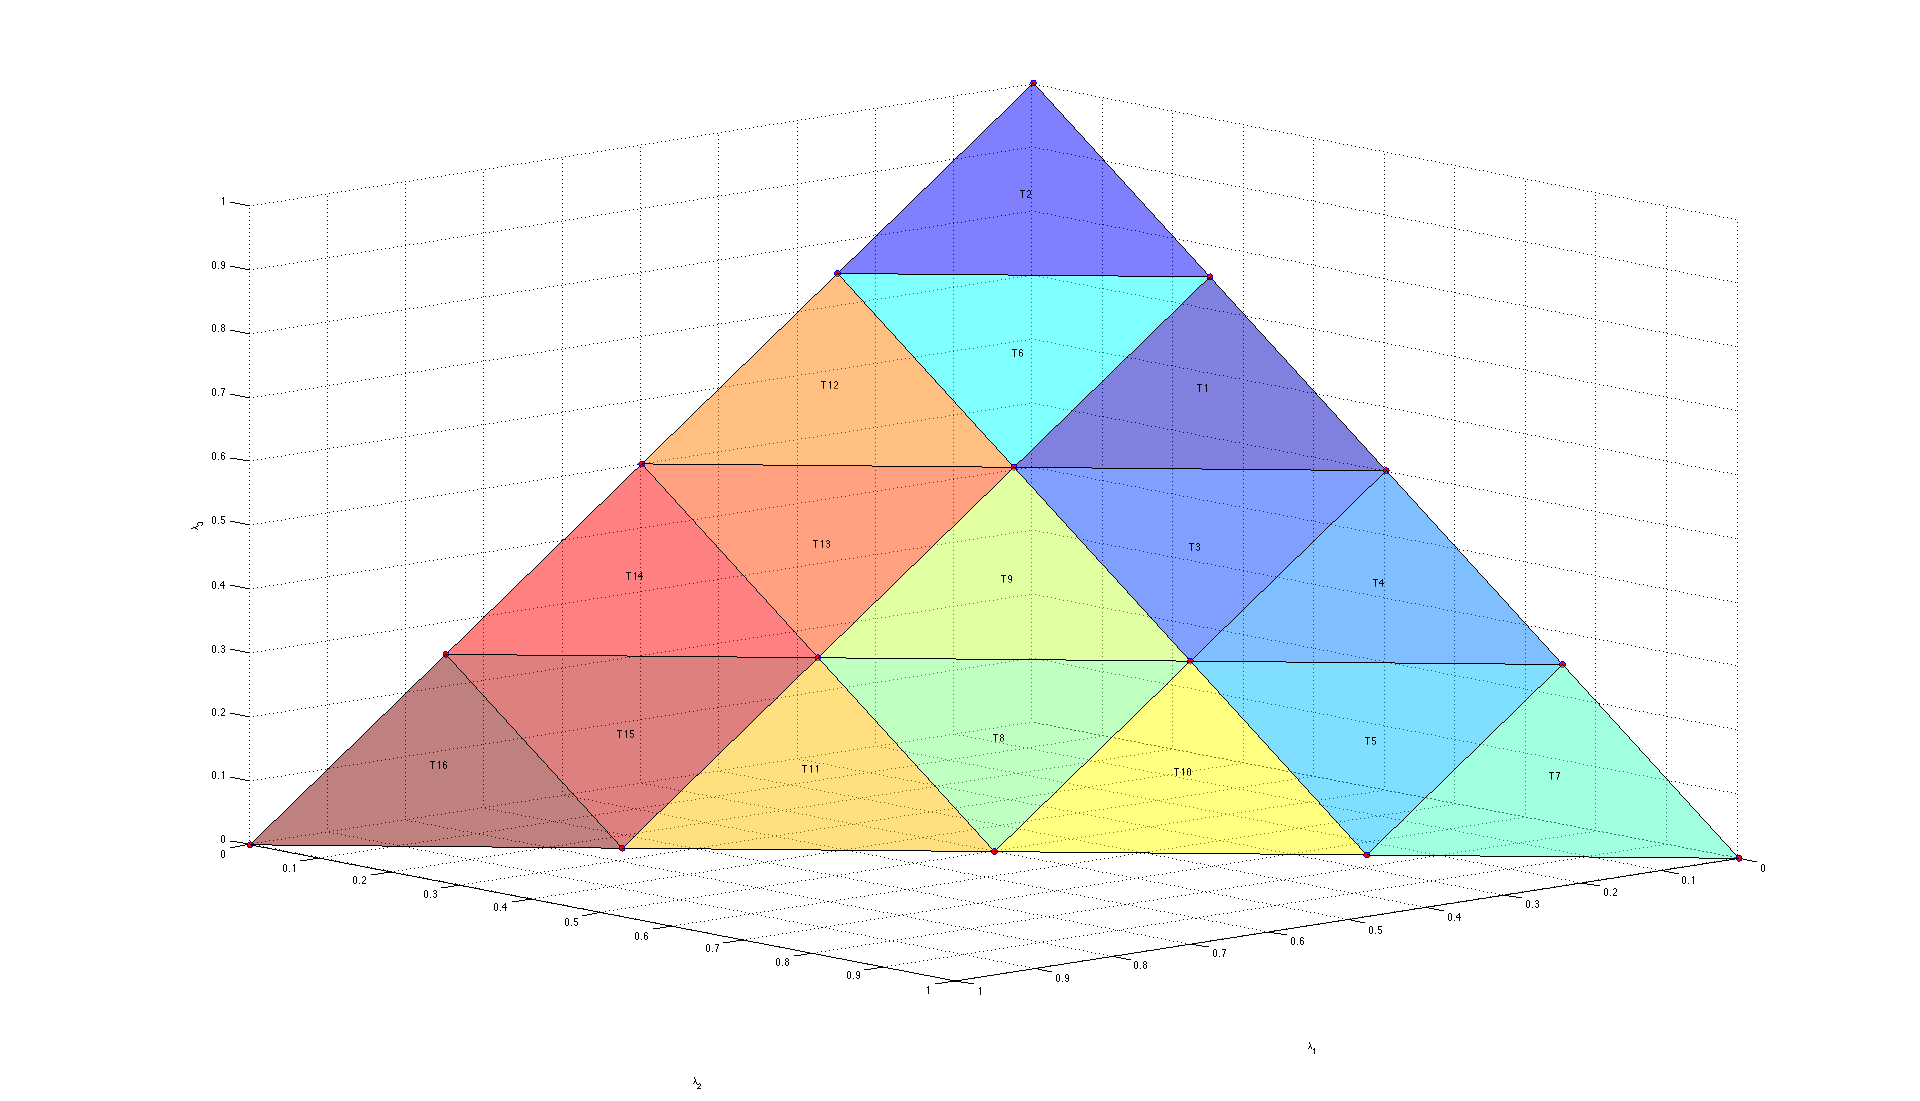
\includegraphics[width=0.900\linewidth]{partition.png}
\caption{Example state-space partition scheme $(N_z = 3, K = 16)$}\label{statespace:figure-partition}\end{figure}


\chapter{Actions and Transitions}
\label{actions_transitions::doc}\label{actions_transitions:actions-and-transitions}
Let $\tilde{A} \ni a_{j}$ denote the finite action set of each individual (small)
player $j \in \mathcal{Z}$. Then $A := \tilde{A}^{\mathcal{Z}} \ni a$, denotes the
$N_{z}$-copies of an individual's action space---i.e. the set of action
profiles $a$. The finite  set $A$ has $N_{a} := |A|$ number of
action profiles.

For each action profile $a \in A$, its associated Markov transition
probability function is a linear operator $P(a): D \rightarrow D$.
\setbox0\vbox{
\begin{minipage}{0.95\linewidth}
\textbf{Relevant functions $\blacktriangleright$}

\medskip

\index{A\_ProfileSet() (built-in function)}

\begin{fulllineitems}
\phantomsection\label{actions_transitions:A_ProfileSet}\pysiglinewithargsret{\bfcode{A\_ProfileSet}}{\emph{self}}{}
Returns the finite set $A$ of $N_{a}$ action profiles
of individual small players. A numeric array of size $N_{a} \times N_{z}$.

\end{fulllineitems}

\index{TransProbA() (built-in function)}

\begin{fulllineitems}
\phantomsection\label{actions_transitions:TransProbA}\pysiglinewithargsret{\bfcode{TransProbA}}{\emph{self}}{}
Returns the finite set of Markov maps $P(a): D \rightarrow D$, one
for every $a \in A$. A numeric array of size $N_{z} \times
N_{z} \times N_{a}$.

\end{fulllineitems}

\end{minipage}}
\begin{center}\setlength{\fboxsep}{5pt}\shadowbox{\box0}\end{center}


\chapter{Intersections with State-space Partitions}
\label{intersections:intersections-with-state-space-partitions}\label{intersections::doc}
For every $k \in \mathbf{K}$ and its associated simplicial partition element $Q_{k} \subset D$ with
positive volume, the
set-valued image $P(a)(Q_{k})$:
\begin{enumerate}
\item {} 
is another $N_{z}$-simplex contained in the unit $N_{z}$-simplex $D$; and

\item {} 
intersects with:
\begin{itemize}
\item {} 
at least one partition element $Q_{k'}$ where $k' \in \mathbf{K}$ and

\item {} 
at most all partition elements $Q_{1}, ..., Q_{K}$;

\end{itemize}

\end{enumerate}


\section{Polytope intersection problems}
\label{intersections:polytope-intersection-problems}\label{intersections:xpoly}
Denote
\begin{gather}
\begin{split}\mathbf{I}(a,k) := \left\{ k' \in \mathbf{K} :
                           P(a)(Q_{k}) \cap Q_{k'} \neq \emptyset
                   \right\},
                   \qquad
                   \forall a \in A, k \in \mathbf{K},\end{split}\notag\\\begin{split}\end{split}\notag
\end{gather}
as the sets of indexes to respective partition-elements---i.e. $k'
\mapsto Q_{k'}$---that contain non-empty
intersections with each simplicial image $P(a)(Q_{k})$. Each nonempty
intersection, induced by each $(a,k) \in A \times \mathbf{K}$ and $P(a)$, is described by
\begin{gather}
\begin{split}Poly_{k'(a,k)} := \left\{ \lambda' \in D :
                             \lambda' \in P(a)(Q_{k}) \cap Q_{k'}
                             \neq \emptyset
                             \text{ and }
                             k' \in \mathbf{I}(a,k)
                     \right\}.\end{split}\notag\\\begin{split}\end{split}\notag
\end{gather}
\begin{notice}{note}{Note:}
Each intersection $Poly_{k'}$, for each
$k \in \mathbf{K}$ and each $a \in A$, is a
\emph{polytope}, and is \emph{at least a simplex}, and is a subset of partition
element $Q_{k'}$, where $k' := k'(a,k)$.
\end{notice}

These nonempty intersections are such that
\begin{gather}
\begin{split}\bigcup_{k' \in \mathbf{I}(a,k)} Poly_{k'} :=: P(a)(Q_{k}).\end{split}\notag\\\begin{split}\end{split}\notag
\end{gather}\setbox0\vbox{
\begin{minipage}{0.95\linewidth}
\textbf{Example}

\medskip


If $N_{z} = 3$, then $D$ is a unit 2-simplex, and
each $Poly_{k'}$ can be a polygon or a triangular subset in $D$.
\end{minipage}}
\begin{center}\setlength{\fboxsep}{5pt}\shadowbox{\box0}\end{center}


\chapter{Sampling on State-space Partitions}
\label{sampling:sampling-on-state-space-partitions}\label{sampling::doc}
We will be drawing uniform sample vectors of the variable $\lambda \in D$ from each partition element $Q_{k},k \in \mathbf{K}$ of the domain $D$. And then we will also use this in conjunction with the {\hyperref[intersections:xpoly]{\emph{Polytope intersection problems}}}.

Each partition element in general is a tetrahedron simplex. We utilize a modified Markov-chain Monte Carlo sampler called the \textbf{Hit-and-Run Algorithm}, originally due to {\hyperref[sampling:smi1984]{{[}Smi1984{]}}}. This algorithm has a desirable property that it can (globally) reach any point in any arbitrarily given bounded set in $\mathbb{R}^n$ in one step. That is, there is a positive probability of sampling from any neighborhood in that set. Moreover, it is proven by {\hyperref[sampling:lov1999]{{[}Lov1999{]}}} that the Hit-and-Run sampler converges fast (in probability) to a uniform distribution on convex bodies $Q_k \subset \mathbb{R}^n$. \footnote{
{\hyperref[sampling:lov1999]{{[}Lov1999{]}}} proves that the upper bound on the convergence rate is in
polynomial time of $\mathcal{O}(n^3)$.
} {\hyperref[sampling:lv2003]{{[}LV2003{]}}} note that this algorithm is the fastest in practice.
\setbox0\vbox{
\begin{minipage}{0.95\linewidth}
\textbf{Hit-and-Run Algorithm}

\medskip


Let $S \subset \mathbb{R}^n$ be a convex region that restricts sample
realizations.
The aim is to generate sample $X := \{ s_m \}_{m=1}^{N_{sim}}$ as a Markov Chain that is (asymptotically) uniformly distributed on $S$. Define $f(s)$ by \emph{any} continuous and strictly positive probability density function (pdf) on $S$.
\begin{itemize}
\item {} 
Start at a given point $s$ in the given set $S$. Let
$m=1$.

\item {} 
Propose a new location $s' = s + l d$ by stepping away from $s$
according to a random direction-stepsize pair, $(d,l)$, where the
direction $d$ is uniformly distributed on the unit hypersphere
$\mathbb{S}^{n-1}$ embedded in
$\mathbb{R}^n$; and the stepsize $l \in \mathbb{R}$ is drawn
from a \emph{proposal density} $g_m(l | d, s)$.

\item {} 
Accept proposal move to $s'$ with \emph{acceptance probability}
$\tilde{\alpha}_f(s,s')$, or, reject and stay at $s$ (i.e. set $s' = s$) with probability
$1-\tilde{\alpha}_f(s,s')$.

\item {} 
Then set $s_{m+1}$ as $s'$, and, repeat the procedure again from
the first step, and let $m = m + 1$.

\end{itemize}
\end{minipage}}
\begin{center}\setlength{\fboxsep}{5pt}\shadowbox{\box0}\end{center}

To implement this simple algorithm, we need to define the functions $\{ g_m(\cdot | d,s) : m \geq 1 \}$, and $f$ (which implies $\tilde{\alpha}_f$) to ensure the necessary and sufficient (Kolmogorov) detailed balance condition holds (for the chain to be a \emph{reversible Markov chain}):
\begin{quote}
\begin{gather}
\begin{split}g_m \left( \| s - s' \| ; \frac{s' - s}{\| s - s' \|}, s
\right) \tilde{\alpha}_f(s,s')f(s) =
g_m \left( \| s - s' \| ; \frac{s - s'}{\| s - s' \|}, s'
\right) \tilde{\alpha}_f(s',s)f(s').\end{split}\notag\\\begin{split}\end{split}\notag
\end{gather}\end{quote}

This demands that the products of probabilities around every closed loop are the same in both directions around the loop.
\begin{itemize}
\item {} 
We can define $f(s)$ by \emph{any} continuous and strictly positive
probability density function (pdf) on $S$.

\item {} 
Let $L_m := \left\{ l \in \mathbb{R} : s_m + l d_m \in S
\right\}$. Define a conditional \emph{proposal density} for each step $m = 1,...,N_{sim}$ by $g_m ( l | d, s)$.
\begin{itemize}
\item {} 
Proposal densities that satisfy the \emph{detailed balance condition} include the class of symmetric proposal density---i.e. $g_m ( l | d, s) = \tilde{g}_m (l) = \tilde{g}(-l)$ for all $l \in \mathbb{R}$,  in which case
\begin{quote}
\begin{gather}
\begin{split}\tilde{\alpha}(s,s') = \min \left\{ \frac{f(s')}{f(s)} ,
1\right\}.\end{split}\notag\\\begin{split}\end{split}\notag
\end{gather}\end{quote}

\item {} 
Since we have also $S$ bounded, we can define a valid proposal
density as
\begin{quote}
\begin{gather}
\begin{split}\tilde{g}_m (l) =  \frac{ \mathbf{1}_{ \{ l \in L_m \} } }{ \int_{\mathbb{R}} \mathbf{1}_{\{ u \in L_m \} } du }.\end{split}\notag\\\begin{split}\end{split}\notag
\end{gather}\end{quote}

\end{itemize}

\end{itemize}
\setbox0\vbox{
\begin{minipage}{0.95\linewidth}
\textbf{Example}

\medskip


In our application, we will define a $S := Q_k$ for every $k \in \mathbf{K}$.
\end{minipage}}
\begin{center}\setlength{\fboxsep}{5pt}\shadowbox{\box0}\end{center}

See Section 6.3.1 of {\hyperref[sampling:ktb2011]{{[}KTB2011{]}}} for a generalized version of this simple algorithm.
\setbox0\vbox{
\begin{minipage}{0.95\linewidth}
\textbf{Looking ahead}

\medskip


Here we give a preview of the usage of uniform sampling from the convex partition elements. In {\hyperref[payoff_approximation::doc]{\emph{Equilibrium Payoff Correspondence}}} later, we show that in our class of dynamic games,
the description of the \emph{symmetric sequential equilibrium} operator (which is correspondence valued) involves solving many \emph{non-separable} bilinear programs (BLP) of the form:
\begin{quote}
\begin{eqnarray*}
\max_{\lambda,w} & u^{T} + \lambda^{T} Q w
\\
s.t. & \lambda \in \mathcal{F}_1(w),
\\
     & w \in \mathcal{F}_2(\lambda);
\end{eqnarray*}\end{quote}

where $u \in  \mathbb{R}^{N_{z}}$ is a vector of constants; $\lambda,w \in \mathbb{R}^{N_{z}}$ are the variables of interest; $Q$ is some $(N_z \times N_z)$ real matrix; and the constraint sets $\mathcal{F}_1(w)$ and $\mathcal{F}_2(\lambda)$ are convex polytopes which, respectively, depend on the choices of $w$ and $\lambda$. \footnote{
A special (and textbook case) is where $\mathcal{F}_1(w) \equiv \mathcal{F}_1$ and $\mathcal{F}_2(\lambda) \equiv \mathcal{F}_2$---i.e. each constraint set $\mathcal{F}_1$ and $\mathcal{F}_2$ do not vary, respectively, with the choice variables $w$ and $\lambda$. This special case is known as a \emph{separable bilinear} program, and, it nests quadratic programming as another special case. These problems are known to have a global solution--see {\hyperref[sampling:bm1993]{{[}BM1993{]}}}. Furthermore, successive approximation using branching-and-bounding methods--i.e. branching into subsets of the optimizer domain, then bounding the value function below by the solutions of linear programs on each subset of the function domain, and, above by the value from a local nonlinear optimizer--can be used to find the $\epsilon$-global optimum: {\hyperref[sampling:mcc1976]{{[}McC1976{]}}} , {\hyperref[sampling:bm1993]{{[}BM1993{]}}} and {\hyperref[sampling:ht1996]{{[}HT1996{]}}}
} \footnote{
In the paper, we noted that in this class of games, the \emph{source of
bilinear nonseparability in the constraint sets} of $\lambda$ and $w$ is
the utilitarian government's set of \emph{incentive} or \emph{promise-keeping} constraints.
}

We propose a Monte Carlo or stochastic approach to obtain $\epsilon$-global (i.e. approximately global) optimization solutions to these non-separable bilinear programs. For now, notice that for each given realization of the random vector $\lambda$, the nonseparable  BLP above can be reduced to standard linear programs (LP) in the variable $w$. \footnote{
Note that by fixing each $\lambda$, the constraint set $\mathcal{F}_1(w)$ will be redundant in the LP formulation within the stochastic global optimization scheme. Additionally, we will also require each realization $\lambda$ to be feasible according to some feasibility (e.g. a budget-balance) requirement(s): $\lambda \in \mathcal{F}(Q_k) := \{ \lambda \in Q_k : \lambda b^{T} \geq 0, \forall b \in B \}$, where $B$ is some finite set of action profiles of the large (government) player.
}
\end{minipage}}
\begin{center}\setlength{\fboxsep}{5pt}\shadowbox{\box0}\end{center}
\setbox0\vbox{
\begin{minipage}{0.95\linewidth}
\textbf{Example (Sampling from $Q_k$ and $Poly_{k'}$)}

\medskip


The following figure ({\hyperref[sampling:figure-intersectsim]{\emph{Uniform samples and various polytope intersections }}}) shows an example of our usage of the Hit-and-Run algorithm in conjunction with our polytope intersection problems described earlier. For example, consider the (4,1)-panel in this figure. It shows the realizations of the random vectors $\lambda P(a)$, where $a = 4$ denotes the fourth action profile in $A$, that would end up in the various partition elements of $(Q_3, Q_4, Q_5, Q_8)$, and given that each vector $\lambda$ is randomly drawn from the set $Q_9$.
\end{minipage}}
\begin{center}\setlength{\fboxsep}{5pt}\shadowbox{\box0}\end{center}
\begin{figure}[htbp]
\centering
\capstart

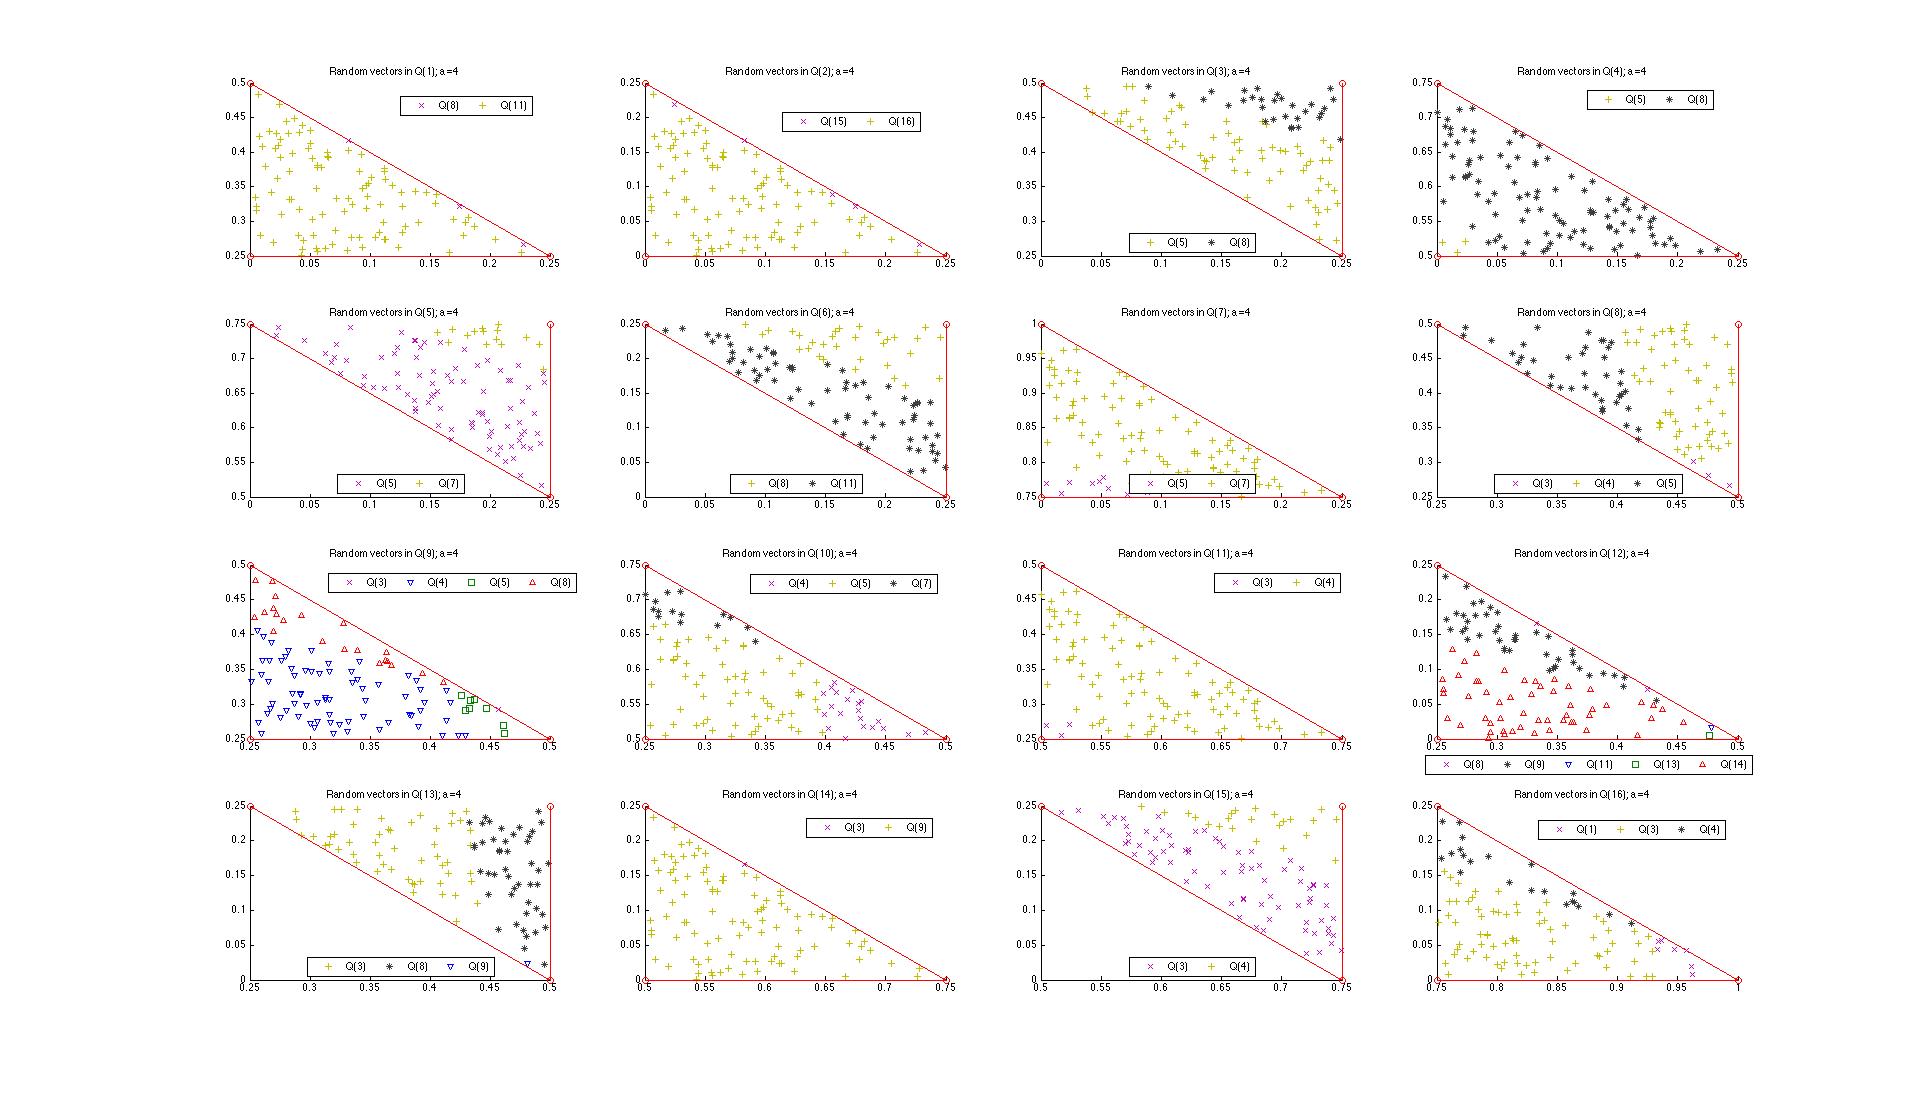
\includegraphics[width=1.000\linewidth]{intersectsim_a4.png}
\caption{Uniform samples and various polytope intersections $(P(a_{4}), N_z = 3, K = 16)$}\label{sampling:figure-intersectsim}\end{figure}

\begin{DUlineblock}{0em}
\item[] 
\item[] 
\item[] 
\item[] 
\item[] 
\end{DUlineblock}


\chapter{State Space Computations}
\label{compute_statespace::doc}\label{compute_statespace:state-space-computations}
Now we describe the implementation for the key tasks involved so far. We will need to:
\begin{itemize}
\item {} 
compute state state partitions: $D := \cup_{k=1}^{K}Q_k$;

\item {} 
construct transitions from each subspace $Q_k$ into corresponding sets
$P(a)(Q_k) \subset D$, for every possible action profile $a \in A$;

\item {} 
record intersections $P(a)(Q_k) \cap Q_k'$, for every $k,k' \in \mathbf{K}$; and

\item {} 
sample uniform points from each $Q_k$, and check for nonempty samples that end up transitioning to each respective intersecting set $P(a)(Q_k) \cap Q_k'$.

\end{itemize}


\section{Storage}
\label{compute_statespace:storage}
We only need to store:
\begin{enumerate}
\item {} 
each index $k' \in \mathbf{I}(a,k) \subseteq \mathbf{K}$, which refers to some partition element(s) $Q_{k'}$ whose subset $Poly_{k'}$ is accessible from $Q_{k}$ given operator $P(a)$.
\begin{itemize}
\item {} 
This suffices for indexing the correct slices of equilibrium payoff sets over the corresponding subset $Poly_{k'}$ of the state space $D$.

\end{itemize}

\item {} 
the finite number of vertices of each $Poly_{k'}$ and the corresponding linear (weak) inequality representation of each $Poly_{k'}$.
\begin{itemize}
\item {} 
This will become apparent later when we solve \emph{separable} bilinear programming problems where it involves optimizing over these subsets $Poly_{k'}$ (when constructing max-min punishment values in the game).

\end{itemize}

\item {} 
the sub-samples from all the Hit-and-Run realizations that belong to every partition element
$Q_k$ which will end up in particular intersections summarized by
each polytope $Poly_{k'}$.

\end{enumerate}


\section{Implementation}
\label{compute_statespace:implementation}
Since we have finite partition elements $Q_{k}$ and finite action
profile set $A \ni a$, then we can enumerate and store all intersections
previously denoted by $\{ Poly_{k'(k,a)}: \forall a \in A, k \in
\mathbf{K} \}$ or equivalently by their index sets $\{ \mathbf{I}(a,k):
(a,k) \in A \times \mathbf{K} \}$.
\setbox0\vbox{
\begin{minipage}{0.95\linewidth}
\textbf{Pseudocode}

\medskip


\begin{DUlineblock}{0em}
\item[] \textbf{For each} $(a,k)\in A \times \mathbf{K}$:
\end{DUlineblock}
\begin{itemize}
\item {} 
Get vertex representation of $Q_k \in D$

\item {} 
Set $P(a)$ as $P$

\item {} 
Get vertex representation $T$ from $P(Q_k)$

\item {} \begin{description}
\item[{Simulate Hit-and-Run uniform realizations in simplex $T$. Get}] \leavevmode\begin{gather}
\begin{split}X := \{ \lambda_n \}_{n=1}^{N_{sim}} \leftarrow RandomPolyFill(N_{sim},T)\end{split}\notag\\\begin{split}\end{split}\notag
\end{gather}
\end{description}

\item {} 
Set $i \leftarrow 0$
\begin{quote}

\begin{DUlineblock}{0em}
\item[] \textbf{For each} $k' \in \mathbf{K}$:
\end{DUlineblock}
\begin{itemize}
\item {} 
Get vertex representation of $Q_k' \in D$

\item {} 
Get intersection $InterPoly = Q_{k'} \cap T$ (a polytope) as:

\end{itemize}
\begin{gather}
\begin{split}InterPoly \leftarrow PolyBool(Q_{k'},T)\end{split}\notag\\\begin{split}\end{split}\notag
\end{gather}\begin{itemize}
\item {} 
If $InterPoly \neq \emptyset$:
\begin{quote}
\begin{itemize}
\item {} 
Set $i \leftarrow i + 1$

\item {} 
Store index to partition elements $Q_{k'}$ when $InterPoly$ is nonempty. Set

\end{itemize}
\begin{gather}
\begin{split}TriIndex(a,k)(i) \gets k'\end{split}\notag\\\begin{split}\end{split}\notag
\end{gather}\begin{itemize}
\item {} 
Store vertex data of polytope. Set:

\end{itemize}
\begin{gather}
\begin{split}PolyVerts(a,k,k') \gets Interpoly\end{split}\notag\\\begin{split}\end{split}\notag
\end{gather}\begin{itemize}
\item {} 
Store linear inequality representation of the same polytope. Set:

\end{itemize}
\begin{gather}
\begin{split}PolyLcons(a,k,k') \gets Vert2Lcon(InterPoly)\end{split}\notag\\\begin{split}\end{split}\notag
\end{gather}\begin{itemize}
\item {} 
Map Monte Carlo realizations $X$ under operator $P$. Set:

\end{itemize}
\begin{gather}
\begin{split}Y \gets P(X)\end{split}\notag\\\begin{split}\end{split}\notag
\end{gather}\begin{itemize}
\item {} 
List members of $Y$ that end up in $InterPoly$. Set:

\end{itemize}
\begin{eqnarray*}
Y_{in} & \gets & InPolytope(Y, InterPoly)
\\
\{ PolyRand(a,k,k'), in \} & \gets & Y_{in}
\end{eqnarray*}\begin{itemize}
\item {} 
Record all vectors $\{\lambda_{n}\} \subseteq X$ that induce $Y_{in}$ under map $P(a)$:

\end{itemize}
\begin{gather}
\begin{split}\{PolyQjRand(a,k,k'), Index\} \gets X(in)\end{split}\notag\\\begin{split}\end{split}\notag
\end{gather}\begin{itemize}
\item {} 
Store corresponding indices $\{n : \lambda_n P(a)\in Y_{in}\}$:

\end{itemize}
\begin{gather}
\begin{split}PolyIndexQjRand(a,k,k') \gets Index\end{split}\notag\\\begin{split}\end{split}\notag
\end{gather}\end{quote}

\end{itemize}
\end{quote}

\item {} 
\textbf{Return}: $TriIndex, PolyVerts, PolyLcons, PolyRand, PolyQjRand, PolyIndexQjRand$

\end{itemize}
\end{minipage}}
\begin{center}\setlength{\fboxsep}{5pt}\shadowbox{\box0}\end{center}

\begin{notice}{note}{Note:}
Computationally, we only need to construct sets $\{
Poly_{k'(k,a)}: \forall a \in A, k \in \mathbf{K} \}$ (e.g. \emph{PolyVerts} and
\emph{PolyLcons} in the pseudocode above) or $\{ \mathbf{I}(a,k): (a,k) \in A
\times \mathbf{K} \}$ (i.e. \emph{TriIndex} in the pseudocode above) once beforehand.
\end{notice}
\setbox0\vbox{
\begin{minipage}{0.95\linewidth}
\textbf{Relevant functions $\blacktriangleright$}

\medskip

\index{Simplex\_IntersectPmap() (built-in function)}

\begin{fulllineitems}
\phantomsection\label{compute_statespace:Simplex_IntersectPmap}\pysiglinewithargsret{\bfcode{Simplex\_IntersectPmap}}{\emph{self}}{}
Returns 4 possible output:
\begin{itemize}
\item {} 
\emph{QP} :
\begin{itemize}
\item {} 
a structure variable containing all others below.

\end{itemize}

\item {} 
\emph{TriIndex} :
\begin{itemize}
\item {} 
a cell array containing indices $k'(a,k) \in \mathbf{I}(a,k) \subseteq \mathbf{K}$ of partition elements that have non-empty intersections with each simplicial image $P(a)(Q_{k})$.

\end{itemize}

\item {} 
\emph{PolyVerts} :
\begin{itemize}
\item {} 
a cell array, where each cell is an array with rows corresponding to vertices of $Poly_{k'(a,k)}$, a polytope contained in the partition element $Q_{k}$. Each cell element is consistent with the index $k'(a,j) \in \mathbf{I}(a,k) \subseteq \mathbf{K}$ stored in \emph{TriIndex}.

\end{itemize}

\item {} 
\emph{PolyLcons} :
\begin{itemize}
\item {} 
is a set of linear (weak) inequality constraint representation of \emph{PolyVerts}.

\end{itemize}

\item {} 
\emph{PolyRand} :
\begin{itemize}
\item {} 
Realizations of random vectors $\lambda_{s}P(a) \in Q_{k'}$ where $k' \in \mathbf{I}(a,k)$ and $\lambda_{s} \sim \textbf{U}[Q_{k}]$---i.e. is uniformly drawn  from $Q_{k}$ according to a Hit-and-Run algorithm {[} HYPERLINK TO ALGORITHM DESCRIPTION {]}, classified according to each \emph{PolyVerts\{a\}\{k\}\{k'\}}.

\end{itemize}

\item {} 
\emph{PolyQjRand} :
\begin{itemize}
\item {} 
Inverse of \emph{PolyRand}. Each \emph{PolyQjRand\{a\}\{k\}\{k'\}} gives the set of $\lambda_{s} \sim \textbf{U}[Q_{k}]$, where under action profile $a$, the induced vector is $P(a)(\lambda_{s}) \in Q_{k'}$ and $k' \in \mathbf{I}(a,k)$.

\end{itemize}

\item {} 
\emph{PolyIndexQjRand} :
\begin{itemize}
\item {} 
Each \emph{PolyIndexQjRand\{a\}\{j\}} gives the set of indices $\{
s \in \{1,...,N_{sim}\} : s \mapsto \lambda_{s} \in Q_{k}, \lambda_{s}P(a) \in Q_{k'}  \text{ and } k' \in \mathbf{I}(a,k)  \}$. The number of \emph{Monte Carlo simulations} of these uniform vectors subject to each convex body $Q_k$ has to be prespecified as $N_{sim}$.

\end{itemize}

\end{itemize}

\end{fulllineitems}



\strong{See also:}


\textbf{PolyBool}, \textbf{Simplex\_Intersect}, \textbf{Vert2Lcon}, \textbf{RandPolyFill}, \textbf{cprnd}


\end{minipage}}
\begin{center}\setlength{\fboxsep}{5pt}\shadowbox{\box0}\end{center}


\chapter{Equilibrium Payoff Correspondence}
\label{payoff_approximation:equilibrium-payoff-correspondence}\label{payoff_approximation::doc}
In {\hyperref[statespace::doc]{\emph{State Space}}} we constructed a partition of the simplex $D:= \Delta(\mathcal{Z})$. Now, we let $D$ be the domain of the equilibrium payoff correspondence.
The task ahead is to approximate the equilibrium value correspondence $\mathcal{V}: D
\rightrightarrows \mathbb{R}^{\mathcal{Z}}$ using
convex-valued step correspondences.


\section{Background}
\label{payoff_approximation:background}
Notation reminder:
\begin{itemize}
\item {} 
Action profile of small players on $[0,1]$, $a \in A$. (Assume $A$ is a
finite set.) Each small player takes on a \emph{personal state} $j \in
\mathcal{Z} := \{ -N,...,-1,+1,...,+M\}$ at each date $t \in
\mathbb{N}$.

\item {} 
Actions of large player ($G$), $b \in B$. $B := \{b \in
\mathbb{R}^{\mathcal{Z}}: -m \leq b(j) \leq \bar{m}, \text{ for } j > 0,
\text{ and, } 0 \leq b(j) \leq \bar{m}, \text{ for } j < 0, \forall j \in
\mathcal{Z}\}$ is a
finite set and contains vectors $b$ that are physically feasible
(but not necessarily government-budget feasible in all states).

\item {} 
Extended payoff vector space, $\mathbb{R}^{\overline{\mathcal{Z}}}$,
where $\overline{\mathcal{Z}} := \mathcal{Z} \cup \{G\}$.

\item {} 
Probability distribution of small players on finite set
$\mathcal{Z}$, $\lambda \in D := \Delta(\mathcal{Z})$.

\item {} 
Profile of continuation values of agents, $w \in
\mathbb{R}^{\mathcal{Z}}$.

\item {} 
Transition probability matrix at action profile $a$, $P(a)$

\item {} 
Individual $j \in \mathcal{Z}$, given action $a(j)$ faces transition probability distribution, $p^j(a(j)) \in P(a)$

\item {} 
Flow payoff profile, $v_j(a,b):= u(c^b(j))-\phi(a_j)$, where
\begin{itemize}
\item {} 
$v(a,b):=(v_j(a,b))_{j\in \mathcal{Z}}$;

\item {} 
Utility-of-consumption function, $u(\cdot)$; and

\item {} 
Disutility-of-effort/action function, $-\phi(\cdot)$.

\end{itemize}

\item {} 
Public date-$t$ history, $h^t := \{ \lambda^t, x^t, b^{t-1} \}_{t \geq 0}$, where
\begin{itemize}
\item {} 
$\lambda^t = (\lambda_0,...,\lambda_t)$ is a history of agent
distributions up to and include that of date $t$;

\item {} 
$x^t = (x_0,...,x_t)$ where $x_t$ is a date-$t$ realization of the
random variable $X_t \sim_{i.i.d.} \mathbf{U}([0,1])$; and

\item {} 
$b^{t-1} = (b_0,...,b_{t-1})$ is a history of government policy
actions up to the end of date $t-1$ and let $\{b_{-1}\} =
\emptyset$.

\end{itemize}

Also, $h^0 := (\lambda_0, x_0)$.

\end{itemize}
\phantomsection\label{payoff_approximation:def-consistency}\setbox0\vbox{
\begin{minipage}{0.95\linewidth}
\textbf{Definition (Consistency)}

\medskip


Let $\mathcal{W}:D \rightrightarrows \mathbb{R}^{\overline{\mathcal{Z}}}$ be a compact- and convex-valued correspondence having the property that $w(G)= \sum_{j\in\mathcal{Z}}\lambda(j)w(j)$ for all $(\lambda,w)\in\text{graph}(\mathcal{W})$. A vector $(b,a,\lambda',w)\in B \times A \times\Delta(\mathcal{Z}) \times\mathbb{R}^{\overline{\mathcal{Z}}}$ is \textbf{consistent with respect to} $\mathcal{W}$ at $\lambda$ if
\begin{enumerate}
\item {} 
$-\lambda b^{T} \geq 0$;

\item {} 
$\lambda'=\lambda P(a)$;

\item {} 
$w\in\mathcal{W}(\lambda')$; and

\item {} 
For all $j\in\mathcal{Z}$, $a(j)\in\text{argmax}_{a'}\left\{(1-\delta) \left[u(c^b(j))-\phi(a')\right]+\delta\mathbb{E}_{p^j(a')}[w(i)]\right \}$.

\end{enumerate}
\end{minipage}}
\begin{center}\setlength{\fboxsep}{5pt}\shadowbox{\box0}\end{center}
\phantomsection\label{payoff_approximation:def-admissibility}\setbox0\vbox{
\begin{minipage}{0.95\linewidth}
\textbf{Definition (Admissibility)}

\medskip

\begin{description}
\item[{For $(\lambda,b) \in D \times B$ let}] \leavevmode\begin{gather}
\begin{split}\pi(\lambda,b):=\min_{(a',\lambda'',w')}
\left[(1-\delta)\sum_{j\in\mathcal{Z}}\lambda(j)[u(c^b(j))-\phi(a'(j))]
+ \delta\sum_{j\in\mathcal{Z}}\lambda''(j)w'(j)\right],\end{split}\notag\\\begin{split}\end{split}\notag
\end{gather}
\end{description}

subject to $(b,a',\lambda'',w')$ is consistent with respect to $\mathcal{W}(\lambda)$. Let $(\tilde{a}(\lambda,b),\tilde{\lambda}'(\lambda,b),\tilde{w}(\lambda,b))$ denote the solutions to the corresponding minimization problem. A vector $(b,a,\lambda',w)\in B \times A \times D \times\mathbb{R}^{\overline{\mathcal{Z}}}$ is said to be \textbf{admissible with respect to} $\mathcal{W}(\lambda)$ if
\begin{enumerate}
\item {} 
$(b,a,\lambda',w)$ is consistent with respect to $\mathcal{W}(\lambda)$; and

\item {} 
$(1-\delta)\sum_{j\in\mathcal{Z}}\lambda(j)[u(c^b(j))-\phi(a(j))]\delta\sum_{j\in\mathcal{Z}}\lambda'(j)w(j)\geq \max_{b'\in B(\lambda)}\pi(\lambda,b')$, where $B(\lambda) := \{ b \in B :- \lambda b^{T} \geq 0 \}$.

\end{enumerate}
\end{minipage}}
\begin{center}\setlength{\fboxsep}{5pt}\shadowbox{\box0}\end{center}
\setbox0\vbox{
\begin{minipage}{0.95\linewidth}
\textbf{Admissible payoff vectors}

\medskip


The payoff vector defined by an admissible vector $(b,a,\lambda',w)$ at $\lambda$ is given by
\begin{gather}
\begin{split}E_G(b,a,\lambda',w)(\lambda)&=(1-\delta)\sum_{j\in\mathcal{Z}}\lambda(j)[u(c^b(j))-\phi(a(j))]+ \delta\sum_{j\in\mathcal{Z}}\lambda'(j)w(j)
\\
E_j(b,a,\lambda',w)(\lambda)&=(1-\delta) \left[u(c^b(j))-\phi(a(j))\right] + \delta \mathbb{E}_{p^j(a(j))}[w(i)].\end{split}\notag\\\begin{split}\end{split}\notag
\end{gather}
Note that $E_G(b,a,\lambda',w)(\lambda)=\sum_{j\in\mathcal{Z}}\lambda(j)E_j(b,a,\lambda',w)(\lambda)$.
\end{minipage}}
\begin{center}\setlength{\fboxsep}{5pt}\shadowbox{\box0}\end{center}

In the paper, we proved the following:
\setbox0\vbox{
\begin{minipage}{0.95\linewidth}
\textbf{SSE Recursive Operator}

\medskip


A SSE is a strategy profile $\sigma \equiv \{ \alpha_t, \beta_t\}_{t \geq 0}$ such that given initial game state $\lambda_0$, for all dates $t \geq 0$, and all public histories $h^t := \{ \lambda^t, x^t, b^{t-1} \}_{t \geq 0}$, $a := \alpha_t(h^t, b_t)$ and $b := \beta_t(h^t)$, and, if $\mathcal{V}$ is the SSE payoff correspondence, then $\mathcal{V}$ is the largest fixed point that satisfies the recursive operator
\begin{gather}
\begin{split}\mathbf{B}(\mathcal{V})(\lambda):=\text{co}\{E(b,a,\lambda',w)(\lambda)\,\vert\,
(b,a,\lambda',w) &\text{ is admissible w.r.t.} \mathcal{V}(\lambda)\},\end{split}\notag\\\begin{split}\end{split}\notag
\end{gather}
where $\text{co}$ denotes the convex hull of a set.

The object of interest can be found recursively: $\mathcal{V} = \lim_{n
\rightarrow +\infty} \mathbf{B}^n(\mathcal{W}_0)$, for any initial
convex-valued and compact correspondence $\mathcal{W}_0$.
\end{minipage}}
\begin{center}\setlength{\fboxsep}{5pt}\shadowbox{\box0}\end{center}

\begin{notice}{note}{Note:}
Given state $\lambda$ and agent payoff vector
$w \in \mathbb{R}^\mathcal{Z}$ determine a unique corresponding
government payoff given by $\lambda \cdot w$. We can thus ignore the
government payoff when defining the equilibrium value correspondences and
their approximations, and restrict their codomain to
$\mathbb{R}^\mathcal{Z}$.
\end{notice}


\chapter{Approximating SSE operators}
\label{payoff_concept:approximating-sse-operators}\label{payoff_concept::doc}
The goal ahead is to \emph{approximate} and provide computable representations of:
\begin{itemize}
\item {} 
each candidate correspondence $\mathcal{W}: D \rightrightarrows
\mathbb{R}^{\mathcal{Z}}$; and

\item {} 
the operator $\mathcal{W} \mapsto \mathbf{B}(\mathcal{W})$.

\end{itemize}


\section{Conceptual}
\label{payoff_concept:conceptual}
Recall $\{Q_k\,|\,k=1,\ldots ,K\}$ denotes a partition of $D$, so
$D=\bigcup_{k=1}^K Q_k$. An upper hemicontinuous, compact- and
convex-valued correspondence $\mathcal{W}:D \rightrightarrows
\mathbb{R}^\mathcal{Z}$ can be approximated by step-valued correspondences using the following procedures: Letting
   \begin{equation*}
        \omega^o_k (\lambda) :=
        \begin{cases}
        \text{co}\bigcup_{\lambda \in Q_k}\mathcal{W}(\lambda') & \text{if} \ (\lambda) \in Q_k,\\
        \emptyset & \text{otherwise},
        \end{cases}
    \end{equation*}
the correspondence defined by $\mathcal{W}^o(\lambda) :=
\bigcup_{k}\omega^o_k (\lambda)$ gives an \emph{outer step-valued approximation}
of $\mathcal{W}$.

Similarly, letting
    \begin{equation*}
        \omega^i_k (\lambda) :=
        \begin{cases}
         \bigcap_{\lambda \in Q_k}\mathcal{W}(\lambda) & \text{if} \ \lambda \in Q_k,
         \\
        \mathbb{R}^\mathcal{Z} & \text{otherwise},
        \end{cases}
    \end{equation*}
the correspondence defined by $\mathcal{W}^i(\lambda) :=
\bigcap_{k}\omega^i_k (\lambda)$ yields an \emph{inner step-valued approximation}
of $\mathcal{W}$.


\section{Practical}
\label{payoff_concept:practical}
Since the convex-valued approximations
$\mathcal{W}^o$ and $\mathcal{W}^i$ are constant on each partition
element $Q_k$, and there are $K < +\infty$ partition elements, these
approximations can be further approximated by constructing outer and inner
approximations for the sets $\omega^o_k (\lambda)$ and
$\omega^i_k (\lambda)$ using \textbf{convex polytopes}.
Let $\mathbb{S}^{N_z-1} := \left\{x \in \mathbb{R}^{N_z} : \| x \| = 1 \right\}$ be the unit $(N_z - 1)$-sphere where the norm $\| \cdot \|$ is given by $\| x \|_{2} = \left(\sum_{j=1}^{N_z} x_{j}^2\right)^{1/2}$. Suppose we have finite sets of directional vectors: $H := \{ h_l \in
\mathbb{S}^{N_z-1} : l = 1,...,L \}$ and $\tilde{H} := \{ \tilde{h}_l \in
\mathbb{S}^{N_z-1} : l = 1,...,L' \}$.
Let
$\bar{\omega}^o_k (\lambda)$ and $\bar{\omega}^i_k (\lambda)$
denote the corresponding polytope approximations, respectively, of $\omega^o_k (\lambda)$ and
$\omega^i_k (\lambda)$, where
     \begin{equation*}
        \bar{\omega}^o_k (\lambda) :=
        \begin{cases}
         \bigcap_{l=1}^{L}\{ z | h_l \cdot z \leq c_{l}^{o}(k) \} & \text{if} \ \lambda \in Q_k,\\
        \emptyset & \text{otherwise}
        \end{cases},
    \end{equation*}
and,
     \begin{equation*}
        \bar{\omega}^i_k (\lambda) :=
        \begin{cases}
         \bigcap_{l=1}^{L'}\{ z | \tilde{h}_l \cdot z \leq c_{l}^{i}(k) \} & \text{if} \ \lambda \in Q_k,\\
        \emptyset & \text{otherwise}
        \end{cases}.
    \end{equation*}
Let $\bar{\mathcal{W}}^o := \cup_{k \in \mathbf{K}}\bar{\omega}^o_k$
and $\bar{\mathcal{W}}^i :=  \cup_{k \in \mathbf{K}}\bar{\omega}^i_k$ denote the resulting correspondences. One would like the ``true'' correspondence $\mathcal{W}$ to be ``sandwiched'' by polytope ``step-correspondences'' $\bar{\mathcal{W}}^o$ from the outside, and, by  $\bar{\mathcal{W}}^i$ from the inside. \footnote{
This idea of providing both upper- and lower-bounding estimates of a given
correspondence was first proposed by {\hyperref[payoff_compute:jyc2003]{{[}JYC2003{]}}} in the computation of
repeated games. Our proposed method is a modification of {\hyperref[payoff_compute:sy2000]{{[}SY2000{]}}}
who in turn extended {\hyperref[payoff_compute:jyc2003]{{[}JYC2003{]}}} to the computation of value correspondences
in dynamic games. Our
contribution will be in the form of \emph{bilinear programming formulations} as
a practical and computable means of constructing these approximate correspondences.
}
\phantomsection\label{payoff_concept:equation-inner-outer-bound}\begin{gather}
\begin{split}        \bar{\mathcal{W}}^i \subset \mathcal{W}^i
        \subset \mathcal{W} \subset \mathcal{W}^o
        \subset \bar{\mathcal{W}}^o.\end{split}\label{payoff_concept-inner-outer-bound}
\end{gather}
The last statement \eqref{payoff_concept-inner-outer-bound} is only true if the step-correspondence levels $c_{l}^{o}(k)$ and $c_{l}^{i}(k)$ are defined, respectively, as the maximal and minimal levels over each domain partition element $Q_k$, in each direction $h_l \in H$ or $\tilde{h}_l \in \tilde{H}$. \footnote{
In the context of our game, where $\mathcal{W}$ stands for a candidate guess of the equilibrium value correspondence, the last statement \eqref{payoff_concept-inner-outer-bound} is only true if the step-correspondence levels $c_{l}^{o}(k)$ and $c_{l}^{i}(k)$ are defined, respectively, as the \textbf{globally} maximal and minimal values of each nonlinear programming problem (which is defined over each state-space partition element $Q_k$, in each direction $h_l \in H$ or $\tilde{h}_l \in \tilde{H}$) that summarizes the concept of \emph{symmetric sequential equilibrium} of the game.
}

In the next section, we show how to construct these upper- and lower
bounding estimates $c_{l}^{o}(k)$ and $c_{l}^{i}(k)$ by using
stochastic global optimization programs and also \emph{separable} bilinear program
formulations, when $\mathcal{W}$ represents a candidate guess of the
\emph{symmetric sequential equilibrium} payoff correspondence in our class of
games.


\chapter{Bilinear programs and SSE operator}
\label{payoff_bilinear::doc}\label{payoff_bilinear:bilinear-programs-and-sse-operator}
Here we give an overview of our main computational insight and proposed method for constructing the operators $\bar{\mathcal{W}}^o \mapsto \mathbf{B}^{o}(\bar{\mathcal{W}}^o)$, and $\bar{\mathcal{W}}^i \mapsto \mathbf{B}^{i}(\bar{\mathcal{W}}^i)$.

Given a candidate correspondence $\mathcal{W}$, evaluating the \emph{symmetric sequential equilibrium} (SSE) operator at this point in the set of compact and convex-valued correspondences (see Definition 3 in the paper), $\mathbf{B}(\mathcal{W})$, will involve:
\begin{enumerate}
\item {} 
Calculating state-dependent max-min punishment values,
$\pi(\lambda) := \max_{b} \pi(\lambda,b)$.
\begin{itemize}
\item {} 
We show that this is amenable to a \emph{separable} bilinear program (BLP).

\item {} 
We will describe how these BLPs are solved to $\epsilon$-global optimality.

\end{itemize}

\item {} 
Given $\pi (\lambda)$, compute the total-payoff sets supported by action-states-continuation-value tuples, $(b,a,\lambda,w)$, that are \emph{admissible} with respect to $\mathcal{W}$:
\begin{itemize}
\item {} 
We will show that this consists of subproblems that are \emph{non-separable}
BLPs.

\item {} 
These can be solved by a specific stochastic global optimization problem
that involves sub-problems that are \emph{linear programs} (LP).

\end{itemize}

\end{enumerate}

We adapt Steps 1 and 2 above for both outer- and inner-approximations, respectively, yielding  approximate outer- and inner evaluations of the step-correspondence images
$\mathbf{B}^{o}(\bar{\mathcal{W}}^{o})$ and $\mathbf{B}^{i}(\bar{\mathcal{W}}^{i})$.


\chapter{Punishment values and BLPs}
\label{payoff_bilinear_punish:punishment-values-and-blps}\label{payoff_bilinear_punish::doc}
The first step is to construct punishment values over each partition element
of the state space. This will turn out to be amenable to \emph{separable bilinear
programming} formulations.

Punishment payoffs for the large player $G$ are constructed as follows.
\begin{itemize}
\item {} 
For each $a\in A$, define a correspondence $\tilde{{\mathcal{W}}}:D\times A \rightrightarrows \mathbb{R}^\mathcal{Z}$ by
\begin{quote}
\begin{align*}
\tilde{{\mathcal{W}}}(\lambda',a)&:=\{w\in {\mathcal{W}}(\lambda')\,|\, \forall j\in \mathcal{Z}, \forall a'\in \tilde{A}
\\
& \delta[p^j(a')-p^j(a_j)]\cdot w\leq (1-\delta) [\phi(a')-\phi(a_j)]\}.
\end{align*}\end{quote}

\begin{notice}{note}{Note:}
Note $\tilde{\mathcal{W}}$ encodes two requirements:
\begin{itemize}
\item {} 
Continuation values $w$ must be \emph{consistent} with the set $\tilde{\mathcal{W}}(\lambda')$ where $w$ itself enforces the action-continuation-state profile pair $(a,\lambda') \equiv (a,\lambda P(a))$; and

\item {} 
individually, the action-and-promised-value pair $(a_j, w_j)$
are optimal (i.e. ``incentive compatible'').

\end{itemize}
\end{notice}

\item {} 
Next, construct government punishment vectors
\begin{itemize}
\item {} 
$(\check{\pi}_k)_{k=1}^K$, and

\item {} 
$(\hat{\pi}_k)_{k=1}^K$

\end{itemize}
\begin{description}
\item[{by letting}] \leavevmode\phantomsection\label{payoff_bilinear_punish:equation-pival_k}\begin{gather}
\begin{split}\pi(\lambda):=\max_{b\in B} \min_{a,\lambda',w}&[(1-\delta)\lambda\cdot v(a,b)+\delta \lambda'\cdot w],\\
\text{s.t.}\,\,& \lambda'=\lambda P(a),\\
& -\lambda b^T \geq 0,\\
& w\in \tilde{{\mathcal{W}}}(\lambda',a),\end{split}\label{payoff_bilinear_punish-pival_k}\\\begin{split}\end{split}\notag
\end{gather}
\end{description}

Then define: $\check{\pi}_k:=\min_{\lambda\in Q_k}\pi(\lambda)$ and $\hat{\pi}_k:=\max_{\lambda\in Q_k}\pi(\lambda)$.

\end{itemize}

\begin{notice}{note}{Note:}\begin{itemize}
\item {} 
If $\mathcal{W}(\lambda')$ is defined as a convex polytope, then $\tilde{\mathcal{W}}(\lambda',a)$ is also a convex polytope.

\item {} 
Given $(a,b) \in A \times B$, the minimization program \eqref{payoff_bilinear_punish-pival_k} is a mild nonlinear programming problem--i.e. a \emph{separable bilinear programming formulation}--of the following generic form

\end{itemize}
\phantomsection\label{payoff_bilinear_punish:equation-BPseparable}\begin{gather}
\begin{split}\min_{\lambda,w} & u^{T} + \lambda^{T} Q w
\\
s.t. & \lambda \in \mathcal{F}_1,
\\
& w \in \mathcal{F}_2.\end{split}\label{payoff_bilinear_punish-BPseparable}\\\begin{split}\end{split}\notag
\end{gather}\begin{itemize}
\item {} 
Moreover, $\mathcal{F}_1$ and $\mathcal{F}_2$ are disjoint convex and bounded polytopes.

\end{itemize}
\end{notice}
\setbox0\vbox{
\begin{minipage}{0.95\linewidth}
\textbf{Existence of Optimum}

\medskip


If $F_1$ and $F_2$ are bounded then there exists an optimal solution of \eqref{payoff_bilinear_punish-BPseparable}, $(\lambda^{\ast}, w^{\ast})$, such that $\lambda^{\ast} \in \mathcal{F}_1$ and $w \in \mathcal{F}_2$.

See {\hyperref[payoff_bilinear_punish:hpt2000]{{[}HPT2000{]}}} or {\hyperref[sampling:ht1996]{{[}HT1996{]}}}.
\end{minipage}}
\begin{center}\setlength{\fboxsep}{5pt}\shadowbox{\box0}\end{center}
\setbox0\vbox{
\begin{minipage}{0.95\linewidth}
\textbf{Separable BLP is NP-complete}

\medskip


A bilinear program can be solved in NP time.

See {\hyperref[payoff_bilinear_punish:man1995]{{[}Man1995{]}}}.
\end{minipage}}
\begin{center}\setlength{\fboxsep}{5pt}\shadowbox{\box0}\end{center}

\begin{DUlineblock}{0em}
\item[] 
\end{DUlineblock}

Assume that we are solving the minimization problem in \eqref{payoff_bilinear_punish-BPseparable}. We employ a well-known deterministic global optimization algorithm known as branch-and-bound (BNB). First, a \emph{relaxation} of the bilinear program is solved. Typically, this is done by solving inexpensive LPs. {\hyperref[payoff_bilinear_punish:cm2009]{{[}CM2009{]}}} The solution of the relaxed problem yields a lower bound on the globally optimal solution which is a convex lower envelope. The relaxation is then iteratively refined, by refining the domain (feasible sets) and successively eliminating dominated local optima. (This is also a common method in solving integer linear programs.) An upper bound estimate of the optima can be found by using local nonlinear solvers (e.g. SNOPT and IPOPT) over each branch. Thus we have successively improved branching partitions of the domain (i.e. \emph{branching}) and lower- and upper-bounding estimates (i.e. \emph{bounding}) of the $\epsilon$-global optimum.

\begin{notice}{note}{Note:}
The BNB algorithm we use follows {\hyperref[sampling:mcc1976]{{[}McC1976{]}}} and is implemented through the
Bilinear Matrix Inequality BNB interface (BMIBNB) available in Stefan
Lofberg's \href{http://users.isy.liu.se/johanl/yalmip/pmwiki.php?n=Solvers.BMIBNB}{YALMIP}. To solve the local lower-bounding LPs, we use the \href{http://www.gnu.org/software/glpk/}{GNU GLPK} open-source optimizer and to solve the upper-bounding nonlinear programs, we use either \href{http://www.sbsi-sol-optimize.com/asp/sol\_products\_snopt\_desc.htm}{SNOPT} or \href{https://projects.coin-or.org/Ipopt}{IPOPT}.
\end{notice}


\section{Implementing punishment values}
\label{payoff_bilinear_punish:implementing-punishment-values}
The following pseudocode implements the punishment calculations for the
outer-approximation scheme:
\setbox0\vbox{
\begin{minipage}{0.95\linewidth}
\textbf{Pseudocode}

\medskip

\begin{quote}

\textbf{Input}: $H, c, PolyLcons$

\begin{DUlineblock}{0em}
\item[] \textbf{For each} $(Q_k,a,b) \in D \times A \times B$:
\end{DUlineblock}
\begin{itemize}
\item {} 
Markov map $P \gets P(a)$

\item {} 
Simplex $T \gets P(Q_k)$

\item {} 
Get $\mathbf{I}(a,k) := \{ k' \in \mathbf{K}: k' \mapsto Q_{k'}
\in D, Q_{k'} \cap T \neq \emptyset$ \}
\begin{quote}
\begin{itemize}
\item {} 
Uses: \emph{xTriIndex} from \textbf{Simplex\_IntersectPmap}

\end{itemize}

\begin{DUlineblock}{0em}
\item[] \textbf{For each} $k' \in \mathbf{I}(a,k)$:
\end{DUlineblock}
\begin{quote}
\begin{itemize}
\item {} 
Get linear inequality representations of $T \cap Q_{k'}$ as

\end{itemize}
\begin{gather}
\begin{split}(M_{k'}, d_{k'}) \gets xPolyLcons(a,k,k')\end{split}\notag
\end{gather}\begin{itemize}
\item {} 
Get current payoff profile $v(a,b)$

\item {} 
Solve separable BLP

\end{itemize}
\begin{gather}
\begin{split}\check{\pi}(Q_k,a,b,k') &
= \min_{\lambda \in Q_k,w} \lambda [ (1-\delta)v(a,b) + \delta P w ]
\\
s.t. &
\\
M_{k'} (\lambda P)^T & \leq d_{k'}
\\
\lambda b^T & \leq 0
\\
H w & \leq c^{o}(Q_k', \cdot)
\\
\delta[p^j(a')-p^j(a_j)]\cdot w & \leq (1-\delta) [\phi(a')-\phi(a_j)], \  \forall j \in \mathcal{Z}\end{split}\notag
\end{gather}\end{quote}
\end{quote}

\item {} 
Get $\check{\pi}(Q_k,a,b) = \min_{k' \in \mathbf{I}(a,k)} \check{\pi}(Q_k,a,b,k')$.

\end{itemize}
\end{quote}
\begin{itemize}
\item {} 
Get $\check{\pi}(Q_k)  = \max_{b \in B} \min_{a \in A}\check{\pi}(Q_k,a,b)$.

\end{itemize}
\end{minipage}}
\begin{center}\setlength{\fboxsep}{5pt}\shadowbox{\box0}\end{center}

\begin{DUlineblock}{0em}
\item[] 
\end{DUlineblock}

\begin{notice}{note}{Note:}\begin{itemize}
\item {} 
The \emph{separable} constraint sets $\mathcal{F}_1$ and
$\mathcal{F}_2$ for $\lambda$ and $w$, respectively,
are given by constraints in the BLP. These constraint say the following.
\begin{itemize}
\item {} 
$\mathcal{F}_1$: the first two constraints require $\lambda \in Q_k$ to be such that
\begin{itemize}
\item {} 
for each $a \in A, k \in \mathbf{K}$ and $k' \in
\mathbf{I}(a,k)$, the resulting continuation state $\lambda P(a) \in Q_{k'} \cap P(Q_k)$; and

\item {} 
given a fixed policy $b$, the choice over $\lambda$
renders $b$ feasible according the the government budget
constraint;

\end{itemize}

\item {} 
$\mathcal{F}_2$ is given by the requirements that $w$ be
\begin{itemize}
\item {} 
consistent with respect to the step correspondence slice
$\mathcal{W}(k')$ which has constant levels over the partition
element $Q_{k'}$; and

\item {} 
such that $w$ is incentive compatible for all small
agents.

\end{itemize}

\end{itemize}

\item {} 
Constructing the punishment values $\hat{\pi}_k$ for the \emph{inner-approximation} scheme is similar to what we did above in detail for $\check{\pi}_k$. The only differences are

\end{itemize}
\begin{enumerate}
\item {} 
in the second last step of the pseudocode above, replace that line with:
\begin{quote}
\begin{gather}
\begin{split}\hat{\pi}(Q_k,a,b) = \max_{k' \in \mathbf{I}(a,k)} \hat{\pi}(Q_k,a,b,k').\end{split}\notag\\\begin{split}\end{split}\notag
\end{gather}\end{quote}

Of course we should also re-label all the $\check{\pi}$ notation for the punishment value function with $\hat{\pi}$; and

\item {} 
\emph{maximize} over $\lambda \in Q_k$ in the main BLP problem.

\end{enumerate}
\end{notice}

\begin{DUlineblock}{0em}
\item[] 
\end{DUlineblock}
\setbox0\vbox{
\begin{minipage}{0.95\linewidth}
\textbf{Relevant functions $\blacktriangleright$}

\medskip

\index{Punish\_Outer() (built-in function)}

\begin{fulllineitems}
\phantomsection\label{payoff_bilinear_punish:Punish_Outer}\pysiglinewithargsret{\bfcode{Punish\_Outer}}{\emph{self}}{}
Returns:
\begin{itemize}
\item {} 
\emph{pival} :
\begin{itemize}
\item {} 
A $(K \times 1)$ numeric array containing elements
$\check{\pi}(Q_k)$ where $k \in \mathbf{K}$.

\end{itemize}

\end{itemize}

\end{fulllineitems}



\strong{See also:}


\textbf{PunishK}


\index{Punish\_Inner() (built-in function)}

\begin{fulllineitems}
\phantomsection\label{payoff_bilinear_punish:Punish_Inner}\pysiglinewithargsret{\bfcode{Punish\_Inner}}{\emph{self}}{}
Returns:
\begin{itemize}
\item {} 
\emph{pival} :
\begin{itemize}
\item {} 
A $(K \times 1)$ numeric array containing elements
$\hat{\pi}(Q_k)$ where $k \in \mathbf{K}$.

\end{itemize}

\end{itemize}

\end{fulllineitems}



\strong{See also:}


\textbf{PunishK}


\end{minipage}}
\begin{center}\setlength{\fboxsep}{5pt}\shadowbox{\box0}\end{center}

\begin{DUlineblock}{0em}
\item[] 
\item[] 
\item[] 
\end{DUlineblock}


\chapter{Computing approximate SSE payoffs}
\label{payoff_compute:computing-approximate-sse-payoffs}\label{payoff_compute::doc}
Now we are ready to describe the computation of the approximate SSE payoff correspondence. The basic idea is from {\hyperref[payoff_compute:jyc2003]{{[}JYC2003{]}}} who use \emph{linear program} (LP) formulations as the approximation. Our extension illustrates that when we have probability distributions (with finite support) as state variables, the approximate SSE payoff correspondence can be constructed via \emph{bilinear program} (BLP) formulations.

Notation:
\begin{itemize}
\item {} 
Let
\begin{gather}
\begin{split}v_j(a,b) := u(c^b(j))-\phi(a_j)\end{split}\notag\\\begin{split}\end{split}\notag
\end{gather}
\item {} 
Given:
\begin{itemize}
\item {} 
a vector of agent actions $a$,

\item {} 
a government policy vector $b$, and

\item {} 
a vector of continuation payoffs $w$,

\end{itemize}

the vector of agents' expected payoffs is defined by
\begin{quote}
\begin{gather}
\begin{split}E(a,b,w):=((1-\delta)v_j(a,b)+\delta P^j(a_j)\cdot w)_{j\in \mathcal{Z}}.\end{split}\notag\\\begin{split}\end{split}\notag
\end{gather}\end{quote}

\end{itemize}


\section{Outer Approximation: Conceptual}
\label{payoff_compute:outer-concept}\label{payoff_compute:outer-approximation-conceptual}
We can now define the outer approximation $\mathbf{B}^o(\mathcal{W})$.
\begin{itemize}
\item {} 
For each search subgradient $h_l\in H$ and each partition element $Q_k$, let
\begin{quote}
\phantomsection\label{payoff_compute:equation-OuterBLP}\begin{gather}
\begin{split}c^{o+}_l(k):=\max_{(a,b) \in A \times B,\lambda\in Q_k, w}& [h_l \cdot E(a,b,w)],
\\
\text{s.t.}\,\,&\lambda'=\lambda P(a),
\\
& \lambda b^T \leq 0,
\\
& w\in \tilde{\mathcal{W}}(\lambda', a),
\\
& (1-\delta)\lambda \cdot v(a,b)+\delta \lambda' \cdot w\geq \check{\pi}_k,\end{split}\label{payoff_compute-OuterBLP}\\\begin{split}\end{split}\notag
\end{gather}\end{quote}

\item {} \begin{description}
\item[{Then define}] \leavevmode\begin{gather}
\begin{split}\bar{\omega}^{o+}_k (\lambda) :=
\begin{cases}
\bigcap_{l=1}^L \{z\,|\, h_l\cdot z\leq  c^{o+}_l(k)\},& \text{if} \ \lambda \in Q_k,\\
\emptyset, & \text{otherwise}.
\end{cases}\end{split}\notag
\end{gather}
\end{description}

\end{itemize}

\begin{notice}{note}{Note:}
Since $A \times B$ is a finite set of action profiles, we can evaluate the program \eqref{payoff_compute-OuterBLP} as a special class of a nonlinear optimization problem--a \emph{nonseparable} bilinear program (BLP)--for each fixed $(a,b) \in A \times B$. Then we can maximize over the set $A \times B$, by table look-up.
\end{notice}


\section{Outer Approximation: Implementation}
\label{payoff_compute:outer-approximation-implementation}
Now we deal with implementing the idea in {\hyperref[payoff_compute:outer-concept]{\emph{Outer Approximation: Conceptual}}}. The
outer-approximation scheme to construct $\mathbf{B}^o(\mathcal{W}^o)$ in
the set of problems in \eqref{payoff_compute-OuterBLP} is computable by following the
pseudocode below:
\setbox0\vbox{
\begin{minipage}{0.95\linewidth}
\textbf{Pseudocode}

\medskip

\begin{quote}

\textbf{Input}: $H, c, \hat{\pi}, Poly$

\begin{DUlineblock}{0em}
\item[] \textbf{For each} $(Q_k,h_l,a) \in D \times H \times A$:
\end{DUlineblock}
\begin{itemize}
\item {} 
Markov map $P \gets P(a)$

\item {} 
Simplex $T \gets P(Q_k)$

\item {} 
Get Hit-and-Run uniform draws constrained to be in $Q_k$: $X:= \{ \lambda_n \}_{n=1}^{N_{sim}} \gets RandomPolyFill(N_{sim}, T)$

\item {} 
Get feasible set $F \gets F(B,Q_k) := \{ ( \lambda, b) \in Q_k \times B  : \lambda \in X \subseteq Q_k,  -\lambda b^T \geq \mathbf{0} \}$

\item {} 
Get $\mathbf{I}(a,k) := \{ k' \in \mathbf{K}: k' \mapsto Q_{k'}
\in D, Q_{k'} \cap T \neq \emptyset$ \}
\begin{quote}
\begin{itemize}
\item {} 
Uses: \emph{TriIndex} from \textbf{Simplex\_IntersectPmap}

\end{itemize}

\begin{DUlineblock}{0em}
\item[] \textbf{For each} $k' \in \mathbf{I}(a,k)$:
\end{DUlineblock}
\begin{itemize}
\item {} 
Get relevant feasible policy set $F(k'; a,k) \gets \{ (\lambda,b) \in F : \lambda P \in Q_{k'} \}$
\begin{quote}

\begin{DUlineblock}{0em}
\item[] \textbf{For each} $(\lambda,b) \in F(k';a,k)$:
\end{DUlineblock}
\begin{itemize}
\item {} 
Get current payoff profile $v(a,b)$

\item {} 
Solve conditional LP:

\end{itemize}
\begin{gather}
\begin{split} c_{+}^{o}(Q_k,h_l,a,k',\lambda,b) &
 = \max_{w} h_l [ (1-\delta)v(a,b) + \delta P w ]
 \\
 s.t. &
\\
 H w & \leq c^{o}(Q_{k'}, h_l)
 \\
 \delta[p^j(a')-p^j(a_j)]\cdot w & \leq (1-\delta) [\phi(a')-\phi(a_j)], \  \forall j \in \mathcal{Z}
 \\
 -\lambda \delta P w &
 \leq \lambda [ (1-\delta)v(a,b) ] - \check{\pi}(Q_{k})\end{split}\notag
\end{gather}\end{quote}

\item {} 
Get $c_{+}^{o}(Q_k,h_l,a,k') = \max_{(\lambda,b) \in F(k';a,k)} c_{+}^{o}(Q_k,h_l,a, k',\lambda,b)$.

\end{itemize}
\end{quote}

\item {} 
Get $c_{+}^{o}(Q_k,h_l,a) = \max_{k' \in \mathbf{I}(a,k)} c_{+}^{o}(Q_k,h_l,a,k')$.

\end{itemize}
\end{quote}
\begin{itemize}
\item {} 
Get $c_{+}^{o}(Q_k,h_l) = \max_{a \in A} c_{+}^{o}(Q_k,h_l,a)$.

\end{itemize}
\end{minipage}}
\begin{center}\setlength{\fboxsep}{5pt}\shadowbox{\box0}\end{center}

\begin{DUlineblock}{0em}
\item[] 
\item[] 
\end{DUlineblock}

\begin{notice}{note}{Note:}\begin{itemize}
\item {} 
In the pseudocode, we can see that for every fixed $(Q_k,a,k') \in D
\times A \times \mathbf{I}(a,k)$ and every feasible $b$, the nested family of programming problems are \emph{nonseparable bilinear programs} (BLP) in the variables $(\lambda, w)$.

\item {} 
The inner most loop thus implements our Monte Carlo approach to approximately
solve for an $\epsilon$-global solution to the \emph{nonseparable} BLPs.

\item {} 
Conditional on each draw of $\lambda$, this becomes a standard
linear program (LP) in $w$ within each innermost loop of the pseudocode.

\item {} 
Given the set of subgradients $H$, an outer-approximation update on the initial step
correspondence $\mathcal{W}^o$, is now sufficiently summarized by
$\mathcal{W}^{o}_{+} = \mathbf{B}^o(\mathcal{W}^o) \gets (H,c_{+}^{o}(Q_k,h_l),\mathcal{W}^o)$.

\end{itemize}
\end{notice}

\begin{DUlineblock}{0em}
\item[] 
\end{DUlineblock}
\setbox0\vbox{
\begin{minipage}{0.95\linewidth}
\textbf{Relevant functions $\blacktriangleright$}

\medskip

\index{Admit\_Outer\_LPset() (built-in function)}

\begin{fulllineitems}
\phantomsection\label{payoff_compute:Admit_Outer_LPset}\pysiglinewithargsret{\bfcode{Admit\_Outer\_LPset}}{\emph{self}}{}
Returns:
\begin{itemize}
\item {} 
\emph{Cnew} :
\begin{itemize}
\item {} 
A $(L \times K)$ numeric array containing elements
$c_{+}^{o}(Q_k,h_l)$ where $k \in \mathbf{K}$ and $h_l \in
H$ are, respectively, a partition element of the correspondence
domain $D$, and, search subgradient in direction indexed
by $l \in \{1,...,|H|\}$.

\end{itemize}

\end{itemize}

\end{fulllineitems}



\strong{See also:}


\textbf{Punish\_Outer}


\end{minipage}}
\begin{center}\setlength{\fboxsep}{5pt}\shadowbox{\box0}\end{center}


\section{Inner Approximation: Conceptual}
\label{payoff_compute:inner-approximation-conceptual}
We now define the \emph{inner approximation} of the SSE value correspondence operator as $\mathbf{B}^i(\mathcal{W})$ below.
\begin{itemize}
\item {} 
Denote $\tilde{H}(k)$ as a finite set of $\tilde{L}(k)$ spherical codes (to be used as \emph{approximation subgradients}, where each
element is $\tilde{h}_l (k)$ and $\| \tilde{h}_l (k) \|_2 = 1$ for all
$l = 1,...,\tilde{L}$ and $k \in \mathbf{K}$.

\item {} 
Assume an initial inner step-correspondence approximation of some
convex-valued and compact-graph correspondence

\end{itemize}
\begin{gather}
\begin{split}\mathcal{W}^{i} := \bigcup_{Q_k \in D}  \bigcap_{\tilde{h}_l (k) \in \tilde{H}(k)}
\left\{ z \in \mathbb{R}^{\mathcal{Z}} :
\tilde{h}_l (k) z \leq c(Q_k,\tilde{h}_l) \right\}.\end{split}\notag\\\begin{split}\end{split}\notag
\end{gather}\begin{itemize}
\item {} 
Define another finite set of fixed $L$ \emph{search subgradients}, made up also of
spherical codes, $H$, just as in the outer approximation method above. \footnote{
Note that we have to let the \emph{approximation subgradients} $\tilde{H}$ to possibly vary with domain partition elements $Q_k$, as opposed to fixed \emph{search subgradients} in $H$ used in the optimization step. This is because the former is endogenously determined by the extra convex hull operation taken to construct an inner step-correpondence $\mathcal{W}^{i}$ at each successive evaluation of the operator $\mathbf{B}^i$.
}

\item {} 
For each \emph{search subgradient} $h_l\in H$ and each partition element
$Q_k$, let
\begin{quote}
\phantomsection\label{payoff_compute:equation-InnerBLP}\begin{gather}
\begin{split}V^{i+}_l(k):=\min_{\lambda\in Q_k} \max_{(a,b) \in A \times B, w}& [h_l \cdot E(a,b,w)],
\\
\text{s.t.}\,\,&\lambda'=\lambda P(a),
\\
& \lambda b^T \leq 0,
\\
& w\in \tilde{\mathcal{W}^i}(\lambda',a),
\\
& (1-\delta)\lambda \cdot v(a,b)+\delta \lambda' \cdot w\geq \hat{\pi}_k,\end{split}\label{payoff_compute-InnerBLP}\\\begin{split}\end{split}\notag
\end{gather}\end{quote}

Set $V^{i+}_l(k) = -\infty$ if the optimizer set is empty.

\item {} 
In contrast to {\hyperref[payoff_compute:outer-concept]{\emph{Outer Approximation: Conceptual}}}, obtain the following additional
step.
\begin{quote}
\begin{itemize}
\item {} 
Let $(a_{l}^{\ast}(k), b_{l}^{\ast}(k), w_{l}^{\ast}(k))$ denote the maximizers in direction $h_l$ and over domain partition element $Q_k$, that induce the level $V^{i+}_l(k)$ above.

\item {} 
Then the corresponding vector of agent payoffs is

\end{itemize}
\begin{gather}
\begin{split}z^{+}_l (k) := E(a_{l}^{\ast}(k), b_{l}^{\ast}(k), w_{l}^{\ast}(k)).\end{split}\notag\\\begin{split}\end{split}\notag
\end{gather}\begin{itemize}
\item {} 
Define the set of vertices $Z(k) = \{ z^{+}_l (k) : l =
1,...,L \}$ and let $\mathcal{W}^{i+}(k) = \text{co} (Z(k))$.

\end{itemize}
\end{quote}

\item {} 
Update
\begin{quote}
\begin{gather}
\begin{split}Z^{+}(k) = \left\{ z^{+}_l (k) \in Z(k) : z^{+}_l (k) \in \partial\mathcal{W}^{i+}(k) \right\};\end{split}\notag\\\begin{split}\end{split}\notag
\end{gather}\end{quote}

and find approximation subgradients $\tilde{H}^{+}(k) = \{ \tilde{h}^{+}_1(k),...,\tilde{h}^{+}_{\tilde{L}^{+}}(k) \}$ and constants $C^{+}(k) = \{c^{+}_1(k),...,c^{+}_{\tilde{L}^+}(k) \}$ such that
\begin{quote}
\begin{gather}
\begin{split}co(Z^{+}(k)) = \bigcap_{l=1}^{\tilde{L}^{+}} \left\{ z: \tilde{h}_l^{+}(k) z \leq
c^{+}_l (k) \right\},\end{split}\notag\\\begin{split}\end{split}\notag
\end{gather}\end{quote}

and $\mathcal{W}^{i+} = \cup_{k} co(Z^{+}(k)) = \mathbf{B}^i (\mathcal{W}^i)$.

\end{itemize}

\begin{notice}{note}{Note:}
As in the \emph{outer approximation} methods, since $A \times B$ is a
finite set of action profiles, we can evaluate the program \eqref{payoff_compute-InnerBLP}
as a special class of a nonlinear optimization problem--a \emph{nonseparable}
bilinear program (BLP)--for each fixed $(a,b) \in A \times B$. Then
we can maximize over the set $A \times B$, by table look-up. Thus,
the only difference computationally in the \emph{inner approximation} method is
the extra step of summarizing each inner step-correspondence $\mathcal{W}^{i+}$ by
updates on:
\begin{itemize}
\item {} 
approximation subgradients in each $\tilde{H}^{+}(k)$;

\item {} 
levels in each $C^{+}(k)$; and

\item {} 
vertices, $Z^{+}(k)$,

\end{itemize}

for every $k \in \mathbf{K}$.
\end{notice}

\begin{DUlineblock}{0em}
\item[] 
\end{DUlineblock}
\setbox0\vbox{
\begin{minipage}{0.95\linewidth}
\textbf{Relevant functions $\blacktriangleright$}

\medskip

\index{Admit\_Inner\_LPset() (built-in function)}

\begin{fulllineitems}
\phantomsection\label{payoff_compute:Admit_Inner_LPset}\pysiglinewithargsret{\bfcode{Admit\_Inner\_LPset}}{\emph{self}}{}
Returns:
\begin{itemize}
\item {} 
\emph{Znew} :
\begin{itemize}
\item {} 
A $(L \times K)$ numeric array containing elements
$z^{+}_l(k)$ where $k \in \mathbf{K}$ and $l \mapsto h_l \in
H$ are, respectively, a partition element of the correspondence
domain $D$, and, approximation subgradient in direction indexed
by $l \in \{1,...,L\}$.

\end{itemize}

\end{itemize}

\end{fulllineitems}



\strong{See also:}


\textbf{Punish\_Inner}


\end{minipage}}
\begin{center}\setlength{\fboxsep}{5pt}\shadowbox{\box0}\end{center}

\begin{DUlineblock}{0em}
\item[] 
\item[] 
\item[] 
\end{DUlineblock}


\chapter{Software}
\label{index:software}
HARDPIG relies on the following software:
\begin{itemize}
\item {} 
\href{http://www.mathworks.com}{MATLAB} platform

\item {} 
\href{http://users.isy.liu.se/johanl/yalmip/pmwiki.php?n=Solvers.BMIBNB}{YALMIP} BMIBNB global optimization solver
\begin{itemize}
\item {} 
Bilinear Matrix Inequality Branch-and-Bound solver

\end{itemize}

\item {} 
\href{http://www.gnu.org/software/glpk/}{GNU GLPK} linear programming
solver (in ANSI C)

\item {} 
\href{http://www.sbsi-sol-optimize.com/asp/sol\_products\_snopt\_desc.htm}{SNOPT} general-purpose local optimization solver (Fortran)
\begin{itemize}
\item {} 
\href{http://www.scicomp.ucsd.edu/~peg/Software.html}{MATLAB Executable binaries files} for up to 300 variables and 300 constraints available freely from Phillip E. Gill.

\end{itemize}

\end{itemize}

Source codes (in MATLAB) and executables (in C/Fortran) are available from the authors via email.


\chapter{Indices and tables}
\label{index:indices-and-tables}\begin{itemize}
\item {} 
\emph{genindex}

\item {} 
\emph{search}

\end{itemize}

\begin{thebibliography}{KTB2011}
\bibitem[BM1993]{BM1993}{\phantomsection\label{sampling:bm1993} 
Bennett, Kristin and Olvi L. Mangasarian (1993): ``Bilinear Separation of Two Sets in n-Space''. \emph{Computational Optimization and Applications}, 2.
}
\bibitem[HT1996]{HT1996}{\phantomsection\label{sampling:ht1996} 
Horst, Reiner and Hoang Tuy (1996): ``Global Optimization: Deterministic
Approaches''. Springer Verlag.
}
\bibitem[KTB2011]{KTB2011}{\phantomsection\label{sampling:ktb2011} 
Kroese, Dirk P., Thomas Taimre and Zdravko I. Botev (2011): \emph{Handbook of
Monte Carlo Methods}. Wiley Series in Probability and Statistics. Wiley.
}
\bibitem[Lov1999]{Lov1999}{\phantomsection\label{sampling:lov1999} 
Lovasz, Laszlo (1999): ``Hit-and-run Mixes Fast''. \emph{Mathematical Programming}, Ser. A 86, 443-461.
}
\bibitem[LV2003]{LV2003}{\phantomsection\label{sampling:lv2003} 
Lovasz, Laszlo and Santosh Vempala (2003): ``Hit-and-Run is Fast and Fun'',
Technical Report, Microsoft Research, MSR-TR-2003-05.
}
\bibitem[McC1976]{McC1976}{\phantomsection\label{sampling:mcc1976} 
McCormick, Garth P. (1976): ``Computability of Global Solutions to Factorable Nonconvex Programs: Part I. Convex underestimating problems''. \emph{Mathematical Programming}, 10, 147–175.
}
\bibitem[Smi1984]{Smi1984}{\phantomsection\label{sampling:smi1984} 
Smith, Robert L. (1986): ``Efficient Monte-Carlo Procedures for Generating Points Uniformly Distributed over Bounded Regions''. \emph{Operations Research}, 32, 1296-1308.
}
\bibitem[CM2009]{CM2009}{\phantomsection\label{payoff_bilinear_punish:cm2009} 
Carpara, Alberto and Michele Monaci. ``Bidimensional packing by bilinear programming''. \emph{Mathematical Programming Series A}, 118, 75–108.
}
\bibitem[HPT2000]{HPT2000}{\phantomsection\label{payoff_bilinear_punish:hpt2000} 
Horst R, P. Pardalos and N. Thoai (2000): \emph{Introduction to global optimization}. 2nd Edition, Boston: Springer, 2000.
}
\bibitem[HT1996]{HT1996}{\phantomsection\label{payoff_bilinear_punish:ht1996} 
Horst R, Hoang Tuy (1996): \emph{Global Optimization}. 3rd Edition, New York: Springer.
}
\bibitem[Man1995]{Man1995}{\phantomsection\label{payoff_bilinear_punish:man1995} 
Mangasarian, Olvi L. (1995): ``The linear complementarity problem as a separable bilinear program''. \emph{Journal of Global Optimization}, 12, 1–7.
}
\bibitem[JYC2003]{JYC2003}{\phantomsection\label{payoff_compute:jyc2003} 
Judd,  Kenneth L., Sevin Yeltekin and James Conklin (2003): ``Computing Supergame Equilibria''. \emph{Econometrica}, 71(4), 1239-1254.
}
\bibitem[SY2000]{SY2000}{\phantomsection\label{payoff_compute:sy2000} 
Sleet, Christopher and Sevin Yeltekin (2000): ``On the Computation of Value
Correspondences''. Unpublished. KGMS-MEDS, Northwestern University.
}
\end{thebibliography}



\renewcommand{\indexname}{Index}
\printindex
\end{document}
